\chapter{Symbolic knowledge representation}
\label{chapt|krs}

\fxnote{Support material: \emph{What is a knowledge representation} by Davis,
Shrobe and Szolovits,
\url{http://groups.csail.mit.edu/medg/ftp/psz/k-rep.html}}

\section{Knowledge and Robotics}
\label{sect|knowledge}

The idea of \emph{Cognitive Robotics} was coined in the early 1990s by Reiter.
In a chapter on that subject in \emph{Foundations of Artificial
Intelligence}~\cite{Levesque2008}, Levesque reminds about the manifesto they
wrote together in 1998:

\begin{quotation}

    Central to this effort is to develop an understanding of the relationship
    between the knowledge, the perception, and the action of [\ldots] a robot. The
    sorts of questions we want to be able to answer are

    \begin{itemize} 

        \item to execute a program, what information does a robot need to have
        at the outset versus the information that it can acquire \emph{en route}
        by perceptual means?

        \item what does the robot need to know about its environment versus what
        need only be known by the designer?

        \item when should a robot use perception to find out if something is
        true as opposed to reasoning about what it knows was true in the past?

        \item when should the inner workings of an action be available to the
        robot for reasoning and when should the action be considered primitive
        or atomic?

    \end{itemize}

    and so on. With respect to robotics, our goal (like that of many in AI) is
    \emph{high-level robotic control}: develop a system that is capable of
    generating actions in the world that are appropriate as a function of some
    current set of beliefs and desires.

\end{quotation}

Indeed, pervasive knowledge could safely be considered as the prominent
characteristic of cognitive robotics. This chapter is dedicated to an analysis
of what is knowledge for a robot, and what are the important features of
knowledge and knowledge representation that are relevant to cognitive robotics.

The next section attempts to give a practical definition of knowledge for
robotics, with a few of its major characteristics. We then review some existing
material from diverse fields of cognitive robotics to propose our own
\emph{typology} of the needs and characteristics of knowledge representation
for service and interactive robotics. About fifty such items are identified,
defined, and organised in a large set.

We then put into practice this reference by surveying nine systems and
architectures for robots. Their main strengths are underline, in order to
depict the state of the research in knowledge representation for robots.

Finally, we conclude this chapter on symbolic knowledge representation by
briefly presenting a novel API for knowledge manipulation, jointly designed
with several other researchers on knowledge representation.

\paragraph{What do we call "knowledge"?}
\label{sect|on-knowledge}

Since we will discuss at length the concept of knowledge in the context of
robotics in the coming pages, it is useful to make our terminology explicit.

No general agreement on a definition of ``knowledge'' exists. In our context,
we call ``knowledge'' \emph{a set of interrelated logical facts that are
meaningful to the robot executive controller}. By \emph{meaningful} we mean
that can possibly be interpreted to lead to a purposeful action. We will see
that our main challenge while designing a cognitive architecture is furthermore
to make this knowledge as \emph{explicit} as possible.

The relation of \emph{data} and \emph{information} to knowledge is a debated
epistemology question known as the ``DIKW'' hierarchy question. In this thesis,
we will associate data to low-level material like raw sensor output, and
information to uncontextualised symbolic facts.

To give a example, we can imagine a human reading a book while being tracked by
a Kinect sensor: the pose of the human skeleton in the world would be the data,
the fact \concept{looksAt(human, book)} as computed by a geometric reasoning
module would be the information, the fact \concept{looksAt(john,
war\_and\_peace)}, fully grounded and connected to the whole knowledge base of
the robot would be proper knowledge.

This simple example also acknowledge the tight coupling between the symbolic
and the geometric realms: while AI at its origins was mostly a matter of
symbolic models, it has been since recognised that not only that the mind is
not a purely abstract system, disconnected from the physical world, but even
more, the cognition fundamentally rely on its relation to the physical world
(so-called \emph{embodied cognition}. Varela\fixme{cite Varela, F. J.,
Thompson, E., \& Rosch, E. (1991). The embodied mind: cognitive science and
human experience. Cambridge, Mass.: MIT Press.} is one of the main discoverer
of these mechanisms, and coined the concept of \emph{enactivism} as the
theoretical framework that study the links between cognition, embodiment and
actions).

\emph{Knowledge} is for us an \emph{information interpreted in the cultural and
social context of the robot}. In practical terms, knowledge is made of
statements that are \emph{contextualized}, \emph{grounded}, and \emph{limited}
to a domain of validity. These three features have important consequences for
the way a knowledge representation and storage system must be designed. Let us
examine them:

\paragraph{Contextualizing} is the ability for a cognitive system to connect a
fact with a \emph{cultural context}, an \emph{interpretive frame} and the set
of other facts previously acquired by the agent.

Since machines are limited to syntactic (in contrast to semantic)
processing, we are mostly looking for a syntactic (\ie, based on symbols)
matching between concepts representations (in our case, sets of alphanumeric
characters).\fxfatal{il faut sans doute évoquer ici la relation
sémantique/syntactique que propose Choamsky}.

The \textit{cultural context} is a broad set of common, general facts that are
considered widely accepted among the interactors (\eg ``bottles may contain
water''). This knowledge is often referred as \emph{common-sense knowledge}.

By \emph{interpretive frame} we mean that a concept may have different
interpretations depending on the agent, the current situation or the time frame
the statement belongs to. Since a fact in one frame can be different (or even
inconsistent) with a fact in another frame (for instance, one object can be
visible for the robot and invisible for another agent), the underlying
knowledge representation system must properly handle these interpretive
frames.

Note that effectively representing a context is a rather different task than
identifying it. This aspect will be further discussed at the end of this work.

\paragraph{Grounding} corresponds to the identification or creation, and then,
maintenance of a link between the symbol (the syntactic form of knowledge
the computer will manipulate) and its semantic, \ie its meaning, anchored in
the world (the relations between the symbol, the referent of the symbol, and
mediating minds is classically referred as the \emph{semantic triangle}, and has
been extensively studied in linguistic). The issue of grounding is well known
in cognitive science and is summarised by Harnard~\cite{Harnad1990} by this
question: ``how the semantic interpretation of a formal symbol system can be
made intrinsic to the system?''. This issue has a very practical importance in
robotic: for a robot to be both endow with a symbolic representational and
reasoning system, and able to \emph{act} in the physical world, it must ground
its knowledge.

\fixme{cite Coradeshi}


\paragraph{Domain of validity} specifies the scope in which
 information is (believed to be) true. It covers several aspects: temporal,
situational and probabilistic. While related to the previous concept of
\emph{interpretive frames}, the domain of validity addresses the question
whether a fact must be or not considered in a given context. This validity
limitation is not usually carried by the fact itself. In the previous example,
for instance, the robot observes a human sitting at a table.  The fact ``a
human is sitting at the table'' is true only for a limited period of time,
until the human stands up. This period of time is not directly accessible
(the robot does not know how long the human plans to stay), but the
knowledge representation must be able to deal with this uncertainty and
should explicitly label this fact as being limited in time.

To know if a fact is \emph{permanent} or \emph{transitional} (Pollock
\cite{Pollock1998}, page 51) is difficult (especially considering that a
feature may be considered as permanent or not depending of the context: within
the situation ``a family meal'', the fact ``the human is sitting at the
table'' could be considered as permanent. Conversely, ``ground is static'' is
generally considered as a permanent fact, expect if we are talking of planetary
mechanics for instance. The difficulty lies in the selection of the relevant
situation in which reasoning must be carried out at a given time) and have
currently to be defined in the cultural background of the robot.

These three aspects lead us to envisage a knowledge representation system
characterized by the following abilities: 
\begin{itemize}
	\item ground raw information,
	\item render a general cultural background, in the form of common-sense knowledge,
	\item attach interpretive frames to new statements,
	\item add and connect new statements to knowledge already present,
	\item store restrictions on the domain of validity of the knowledge.
\end{itemize}

Besides, the following active processes would be desirable:
\begin{itemize}

    \item acquire and maintain knowledge perceived from the physical world or
        retrieved from other sources (interaction with other agents, web-based
        contents,...)

    \item monitor contexts and accordingly manage the validity of the stored
        knowledge,

    \item ensure the logical consistency of the knowledge repository, and
    explicit inconsistencies when required\footnote{One may argue that the
    real world is however inherently inconsistent; we will discuss several
    aspect of inconsistencies representation and management later on.}.

\end{itemize}

We have already seen in the imaginary scenario introduced in
chapter~\ref{chapt|intro} that many other cognitive abilities related to
knowledge representation and manipulation are required by service robots. The
above items give a high-level view of what knowledge \emph{intrinsically} need
to exist. The next section aims, on the contrary, at providing a
comprehensive set of cognitive abilities related to knowledge.


%%%%%%%%%%%%%%%%%%%%%%%%%%%%%%%%%%%%%%%%%%%%%%%%%%%%%%%%%%%%%%%%%%%%%%%%%%%%%%%%%%%%%%%%%%%
%%%%%%%%%%%%%%%%%%%%%%%%%%%%%%%%%%%%%%%%%%%%%%%%%%%%%%%%%%%%%%%%%%%%%%%%%%%%%%%%
\section{A Typology of Knowledge Representation Requirements for Robotics}
\label{sect|features}

This section now focuses on formalizing the knowledge representation issue: we
aim first at establishing a comprehensive typology and nomenclature
(figure~\ref{fig|taxo}) of representational needs for robotics in the specific
context of service robotics, before painting, at
section~\ref{sect|surveyed-systems}, the current landscape of approaches to the
knowledge representation problem in the research community. For each such
``dimensions'' of knowledge representation system, we provides a short
definition accompanied by links to relevant literature.

\begin{figure}
        \centering
        \includegraphics[width=0.8\columnwidth]{taxonomy.pdf}
        \caption{Taxonomy of the analysis dimensions of knowledge
        representation systems for service robotics.}
        \label{fig|taxo}
\end{figure}

The typology has been built from three main sources: a review of the existing
literature on that topic that we present in the next section; the survey of
nine knowledge representation systems already deployed; our own experience,
acquired during the thesis preparation with the help of many discussions with
researchers from both CNRS and TUM, that allowed to interweave two slightly
different perspectives on knowledge in robotics.

\subsection{Previous Work}
\label{sect|evaluation-literature}

As said, the typology we propose is in part based on a comprehensive synthesis of
classifications and analysis found in the literature. This synthesis is focused
on cognitive abilities strictly related to knowledge manipulation in the
context of service robotics.

Levesque and Lakemeyer~\cite{Levesque2008} present in their chapter on
Cognitive Robotics several characteristics of knowledge representation systems
for robots, stressing the need of representing the \emph{dynamics of the
world}.  Sensing is included in the knowledge representation via
\emph{fluents}; they introduce the idea of \emph{possible worlds} to represent
distinct parallel mental models; action representation and reasoning about
tasks is discussed in the context of \emph{situation calculus}; \emph{open
world} vs. \emph{closed world} approaches are mentioned.  They also discuss how
robot programming and knowledge representation can be related. We integrate
most of these items in our typology.

In a slightly broader context, Heintz et al.~\cite{Heintz2008} define
\emph{knowledge processing middlewares} as systems supporting ``declarative
specifications for flexible configuration and dynamic reconfiguration of
context dependent processing at many different levels of abstraction''. They
identify six characteristics: the system must be able to \emph{merge
informations} from different, possibly distributed sources; it should support
quantitative as well as qualitative processing of information, it should offer
\emph{bottom-up} and \emph{top-down} processing, it should be able to deal with
\emph{uncertainty}, allow for ``flexible configuration and reconfiguration''
(which require what we call here \emph{non-monotonicity}) and finally
\emph{meta-knowledge} and \emph{introspective capacities} (``declarative
specification of the processing functionalities'').

Several surveys compare global cognitive architectures \cite{Langley2006,
Vernon2007, Chong2009}. Langley, Laird and Rogers~\cite{Langley2006}
distinguish nine capabilities: recognition and categorization, decision making,
perception and situation assessment, prediction and monitoring, planning,
reasoning, execution control, interaction and
learning/remembering/introspection. They also separately identify four
\emph{properties} of cognitive architecture, that categorise how knowledge is
handled by the architecture: representation of knowledge, organization of
knowledge, utilisation of knowledge and acquisition and refinement of
knowledge. This categorisation had a notable influence on our typology, and
many of these categories are also present in our proposal.

Vernon et al.~\cite{Vernon2007} split these architectures into two broad
categories: the \emph{cognitivist} ones (where cognition is considered as an
explicit computation problem, often based on symbol manipulation), and the
\emph{emergent} ones (where cognition only exists as a result of the
interaction of the system with its environment). The approaches presented in
this paper are, at a few exceptions, prototypical \emph{cognitivist} approaches
that aim at making knowledge explicit within the robot architecture. Vernon et
al. propose twelve \emph{characteristics of cognitive system} to compare
architectures. Amongst them, they mention the \emph{inter-agent epistemology}
(how the structure of the world is captured in a representation and shared),
the relation to \emph{embodiment}, the ability to \emph{anticipate} and to
\emph{adapt}, and the mechanisms of \emph{motivation}. While presented at the
level of the whole robotic architecture, these features also translate into
knowledge representation strategies and are relevant to our study.

Chong et al.~\ref{Chong2009} also provide a recent review of the main cognitive
architectures, with a focus on eight functions: perception, memory, goals
management, problem solving capabilities, planning, reasoning, learning and
links to neurobiology.

At an even broader scope, several authors from fields that are connected to
robotics have previously listed desirable features of artificial systems aiming
at rich cognitive abilities.

For instance McCarthy recently listed in~\cite{McCarthy2007} the challenges he
identifies on the road to a \emph{human-level AI}.

\begin{itemize}

	\item the ability to \emph{"operate successfully in the common sense
	informatic situation"},

	\item the necessity of relying on mathematical logic, as the most fruitful
	formalism for machine intelligence,

	\item the ability to deal with \emph{approximate concepts and approximate
	theories} (that would include representing them, and reasoning with them),

	\item non-monotonic reasoning,

	\item what McCarthy calls \emph{Elaboration Tolerance}: the ability to
	extend \emph{on demand} the closed domain of interpretation for a
	given assertion,

	\item the ability to formalize and reason about contexts,

	\item reasoning about events, and in particular, actions,

	\item the capacity of introspection,

	\item and finally, he points the issue of giving computer the right
	heuristics for decision making.

\end{itemize}

Coming from the perspective of natural language processing in situated context,
Roy and Reiter summarise in~\cite{Roy2005} what they see as the main challenges
to be tackled by knowledge representation systems: \emph{cross-modal
representation} systems, association of words with perceptual and action
categories (\emph{grounding}), modeling of \emph{context}, definition of the
right \emph{granularity} of models, integration of \emph{temporal modeling and
planning}, ability to \emph{match past (learned) experiences} with the current
interaction and ability to take into account the \emph{human perspective}.

Knowledge representation systems in robotics are directly affected by these
points, and we indeed integrate them in our typology, in slightly reformulated
ways.


\subsection{What Can be Represented?}
\label{sect|expressiveness}

\begin{scriptsize}
\begin{center}
\begin{tikzpicture}[taxonomy]
    \node [taxon] {\bf A. Expressiveness}
            child {node [taxon] {{\bf A.5}. Meta-cognition}}
            child {node [taxon] {{\bf A.4}. Uncertainty}}
            child {node [taxon] {{\bf A.3}. OWA/CWA}}
            child {node [taxon] {{\bf A.2}. Expressive power}}
            child {node [taxon] {{\bf A.1}. Logic formalism}};
\end{tikzpicture}
\end{center}
\end{scriptsize}

This first axis of analysis is its intrinsic expressive power. It answers the
question: what can be possibly represented. When it explicitly exists, the
\emph{language} of representation plays here an obvious role.

\subsubsection{Main Logic Formalisms}

The main role of a knowledge representation system is to provide an adequate
representation system to formally store facts and concepts that could be informally
described in natural language.

Formal logic aims at providing such a representation system with the added
value of providing a tractable support for inference and reasoning.

Most (but not all) of the systems we have surveyed rely on a particular logic
formalism. The choice of the formalism has a strong impact, on one side, on the
range of ideas that can be expressed conveniently (\emph{practical
expressiveness}) or at all (\emph{theoretical expressiveness}), on the other
side, on the ability to solve the fundamental inference problem (called
\emph{satisfiability}: is a given logical sentence true in my model?) in a
tractable manner.

A large number of logic formalism do exist and we briefly present below the most
relevant ones for systems actually deployed in robotic architectures.

\emph{Predicate logic} is the family of logic formalisms the most commonly
found in knowledge representation. It distinguishes itself from the simpler
\emph{propositional logic} by the use of quantification to increase generality.
\emph{First-order logic} (FOL) is the subpart of \emph{predicate logic} where the
objects of \emph{predicates} (or \emph{formulae}) are simple \emph{terms},
while in \emph{higher-order logics}, predicates can be themselves objects of
other predicates.

\emph{Horn clauses} are an important subset of FOL because the satisfiability
of a set of such clauses is a $P$-complete problem (\ie practically tractable).
A Horn clause is a disjunction of literals (a \emph{clause}) with at most one
positive literal: $\neg p \lor \neg q \lor \cdots \lor \neg t \lor u$, which
can also be represented as $(p \land q \land \cdots \land t) \rightarrow u$.
Important logic programming languages like Prolog are based on Horn clauses.

The family of \emph{Description Logics}~\cite{Baader2008} also play an
important role. It is also a subset of the first-order logic, with some
extensions in second-order logic. Description logics are notable because most
of them are known to be decidable (but not always in a practically tractable
manner). In description logic, axioms are build from \emph{concepts},
\emph{roles} (that are unary or binary predicates) and \emph{individuals}. The
W3C OWL-DL standard is a widely-used language to describe domains with the
description logic.

Because description logics have been originally created from the perspective of
a \emph{knowledge representation language} and not a logic language, their
terminology (\emph{concept} or \emph{class}, \emph{role} or \emph{property},
\emph{individual},\ldots) is well-suited to knowledge description.

\emph{Modal logic}, that allows for statement qualification like
\emph{possibility} or \emph{necessity}, have been shown to be closely related
to description logics~\cite{Baader2001}. Modal logic allows to represent conveniently parallel
possible worlds and facts like ``the robot knows \emph{that the human knows}
how to read a recipe''.

\fxfatal{On modal logics, see the remark of McCarthy, in \cite{McCarthy2007}, section 3}

\emph{Temporal logic} are designed to represent and manipulate assertions whose
truth value may vary in time. We introduce one of its key idea (the
\emph{fluents}) later in the typology.

One last class of logics that is of particular relevance for robotic
applications is the \emph{probabilistic logics} or \emph{Bayesian logics}.
These logics provide a formal framework to reason on propositions whose truth
or falsity is uncertain. We elaborate below on the representation of uncertainty.

Note that most of these logic formalisms are still active research field on
their own, and practical considerations (especially the availability of
reasoners efficient enough for on-line use on a robot) often constraint the
choice of a logical formalism and a level of expressive power.

\subsubsection{Expressive Power}

Logical formalisms each bring a certain level of expressive power. For
instance, the following classical syllogism can not be represented in
propositional logic because of the use of \emph{universal quantification}:

\begin{quote}
\begin{enumerate}
    \item All men are mortal,
    \item Socrates is a man,
    \item Therefore, Socrates is mortal
\end{enumerate}
\end{quote}

However, the following weak version of the syllogism can be represented in
propositional logic:

\begin{quote}
\begin{enumerate}
    \item If Socrates is a man, then Socrates is mortal,
    \item Socrates is a man,
    \item Therefore, Socrates is mortal
\end{enumerate}
\end{quote}

Generally speaking, expressive power comes at the cost of more complex
\emph{satisfiability} and \emph{consistency}\footnote{We precise these concepts
at section~\ref{sect|reasoning}.} computations, possibly leading to
untractable, if not undecidable (\ie systems where it is proven that a
proposition can not be decided to be true or false) problems.

\begin{figure}
    \centering
    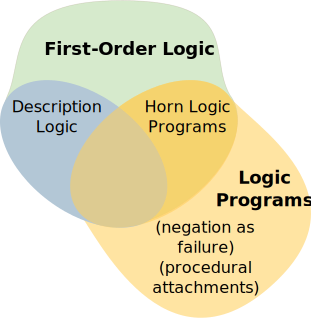
\includegraphics[width=0.3\columnwidth]{typology/expressive_overlap_dl_horn.pdf}
    \caption{expressiveness overlap of Description Logics and logic programs
    based on Horn clauses, taken from~\cite{Grosof2003}}
    \label{fig|overlap_dl_horn}
\end{figure}

Figure~\ref{fig|overlap_dl_horn} shows that the expressive power of description
logics and Horn clauses partially overlaps. In section~\ref{sect|reasoning} we
mention extensions to description logics based on rule systems that bring closer
the two approaches.

The relationships between expressive power and reasoning complexity that follow
has been extensively studied for Description Logics.
Zolin~\cite{ZolinDLComplexityNavigator} maintains a ``complexity navigator''
that allows to conveniently explore these relationships and indexes most of the
literature on that subject.

It can be noted that the relation between expressiveness and reasoning
complexity is fragile: for instance, adding the following axiom \stmt{farFrom
disjointProperty near} (that states that two individuals can not be at the
same time near and far from each other) changes the expressiveness power of
the ORO Common-Sense ontology (presented at chapter~\ref{chapt|oroserver}
from $\mathcal{SHOIQ(D)}$ to $\mathcal{SROIQ(D)}$: this seemingly innocuous
assertion change the complexity class of the whole ontology, and the concept
satisfiability reasoning problem switches from a {\it NExpTime-complete}
problem to a {\it NExpTime-hard} problem (\ie, \emph{at least} as hard as the
hardest problem in {\it NExpTime}).

This ``instability'' has practical consequences on run-time performances on
the robot because a light alteration of the knowledge structure can lead to
very noticeable performance drops.


\subsubsection{Open World and Close World Assumptions}
\label{sect|owa-cwa}

The \emph{close world} (CWA) vs. \emph{open world} (OWA) assumptions name a
modelling choice on the \emph{completeness} of a knowledge domain. In the close
world assumption, a proposition that can not be proven true is assumed to be
false (\emph{negation by failure}), while in the open world assumption, a
proposition may be considered either true, false or unknown.

This distinction is important in robotics where the robot may have to manipulate
concepts with only partial knowledge on them. For instance, let imagine a robot
that sees a bottle on a table, whose bottom is hidden by another object. The
robot can not prove that the bottle is indeed \emph{on} the table. A knowledge
representation system relying on the closed world assumption would then assume
the bottle is \emph{not} on the table ($\lnot R^{CWA}_{isOn}(bottle, table)$)
whereas with the open world assumption, the proposition $R^{OWA}_{isOn}(bottle,
table)$ would be undecided. Example in table~\ref{table|cwa-owa-example} provides
another example of consequences of the CWA/OWA choice on reasoning.

\begin{table}
    \begin{center}
    \begin{tabular}{ll}
    {\bf Action} & {\bf Part involved} \\
    \hline
    {\tt PickSoftly} & hand \\
    {\tt PickAndPlace} & arm, hand \\
    {\tt MoveArm} & arm \\
    \hline
    \end{tabular}
    \end{center}
    \caption{Assuming the question is: \emph{select actions that do not require
    to move the arm}, a CWA reasoner would return {\tt PickSoftly} whereas an
    OWA reasoner would not return anything if the {\tt PickSoftly} action is
    not explicitly said not to involve the arm.}
    \label{table|cwa-owa-example}
\end{table}

The OWL language is specifically known to assume an open world.  Domains
constrained with the closed world assumption lead to more tractable inference
problems, and allow for instance the use of logic languages like Prolog. Thus,
several approaches exists to \emph{locally close} a domain (\cf
Levesque~\cite{Levesque2008}, section 24.3.2 for a summary of those ones).

\subsubsection{Representation of uncertainty and likelihood}

Sources of uncertainty for a robot are two-fold: uncertainty \emph{intrinsic}
to facts (like \emph{``It may rain tomorrow''}), uncertainty caused by
imperfect perception of the world (\emph{``Is the bottle really on the
table?''}). Most logics do not account explicitly for uncertainty. It must be
either relied on specific logics (like Bayesian logics) or on extensions of
classical logics.

\fxwarning{To be completed!}

\subsubsection{Meta-cognition: knowledge on the knowledge}

As stated by Cox and Raja~\cite{Cox2007}, meta-cognition is composed of both
\emph{``meta-level control of cognitive activities and the introspective
monitoring of such activities to evaluate and to explain them"}.

Sloman proposes in~\cite{Sloman2011} a detailed analysis of meta-cognition and
its different aspects in both natural (human) and artificial systems.

A knowledge representation system endowed with \emph{meta-cognition} is not
only able to manipulate knowledge but also to exhibit and manipulate the
structure of its knowledge and the reasoning process. For instance, the ability
to explain a logical inconsistency in a KRS is a meta-cognitive function, as is
the ability to expose and alter the knowledge structure (these two reasoning
techniques have their own entries in the taxonomy, at
section~\ref{sect|reasoning}.

At section~\ref{sect|introspection} below, we discuss the idea of
introspection.  Meta-cognition can be viewed as the technical facet of the
introspection in general.


%%%%%%%%%%
\subsection{How things are represented?}
\label{sect|higher-level-domain-representation}

We do not discuss in this section the general strategies to construct a
knowledge model (they will be presented in
section~\ref{sect|design-strategies}). We focus here on questions that involve
representational challenges (time, space, context) or require specific
cognitive capabilities (theory of mind, introspection, memory).

\begin{scriptsize}
\begin{center}
\begin{tikzpicture}[taxonomy]
    \node [taxon] {\bf B. Representation}
            child {node [taxon] {{\bf B.5}. Memory}}
            child {node [taxon] {{\bf B.4}. Introspection}}
            child {node [taxon] {{\bf B.3}. Modality}}
            child {node [taxon] {{\bf B.2}. Context}}
            child {node [taxon] {{\bf B.1}. Roles}};
\end{tikzpicture}
\end{center}
\end{scriptsize}

\subsubsection{Role Representations}

This section discusses strategies and approaches to represent in a knowledge
model three important \emph{roles}: spatial relations, time and representation
of actions.

\begin{scriptsize}
\begin{center}
\begin{tikzpicture}[taxonomy]
    \node [taxon] {\bf B.1 Roles}
            child {node [taxon] {{\bf B.1.3}. Actions}}
            child {node [taxon] {{\bf B.1.2}. Time}}
            child {node [taxon] {{\bf B.1.1}. Space}};
\end{tikzpicture}
\end{center}
\end{scriptsize}


\paragraph{Representation of space}

Symbolic representation of space is a widely studied topic. In particular, a
large literature corpus is available on spatial ontologies\fxwarning{Which one?}.

Two main classes of spatial relations are usually represented at the symbolic
level: the topology of environments and the placement of physical entities.

\begin{scriptsize}
\begin{center}
\begin{tikzpicture}[taxonomy]
    \node [taxon] {\bf B.1.1 Space}
            child {node [taxon] {{\bf B.1.1.2}. Placement}}
            child {node [taxon] {{\bf B.1.1.1}. Topology}};
\end{tikzpicture}
\end{center}
\end{scriptsize}

\fxwarning{...topology??}

Symbolic representation of entities placement can be absolute or relative. The
relation \concept{isOn}, for example, leads to absolute statements: the
validity of the relation is independent of the nature of its subjects and
objects, and is also independent of the observer.

On the contrary, the relation \concept{nextTo} is relative, and depends on the
relative size of the subject and the object. Two houses distant of 2 meters
from each other can be considered as next to each other. Two ants separated by
2 meters are not next to each other.

The relation \concept{leftOf} is another example of relative spatial relation,
this time because it depends on the observer viewpoint.

\fxwarning{\concept{front}/\concept{back} -> entities have or not a concept of front/back.}

Choices must be made in the knowledge representation system to adequately
represent relative spatial relations. Options include the computation of such
relations only on-demand, when the context is know (which viewpoints, etc.) or
storage of these facts in different models, one per agent.

\fxwarning{Find references on that subject -> classification of spatial
relations. Wikipedia?}

\paragraph{Representation of time}
\label{sect|time-representation}

As an agent acting at human-like time scale and dealing with temporal concepts
(like actions), a robot needs to represent and reason about
time. Time representation is split into two distinct abilities: representing
time points (both in the past -- which is roughly equivalent to assignment of
timestamps to events the robot perceives -- and in the future), and
representing passing time (situations, durations, timespans) like in
\emph{``the eggs will be cooked in 10 min''}.

This is usually formalised as a disjunction in time representation between
\emph{events}, that is, any durationless temporal concept, and
\emph{situations}, that is, any temporal concept with a non-zero
duration\footnote{Other definitions of a situation do exist, notably in the
context of \emph{situation calculus}~\cite{Levesque1998}, Reiter and Levesque
consider a situation to be an history of actions.}.

\fxfatal{Discuss time chronicles~\cite{Ghallab1996}}
\fxfatal{Discuss Allen intervals}

The concept of \emph{fluent} plays another important role for time
representation. Fluents are properties (or \emph{conditions}) that change over
time, like $sees(agent1, apple, t)$.\fxwarning{Un peu court... citation?}

We call a system that does not account for time (\ie that permanently lives in
present) \emph{atemporal}.


\paragraph{Actions}

Events and actions are two temporal concepts that are of particular importance to
robotic systems, as systems that perceive, react and perform in their environment.

While representation of events boils down to label a timestamp,
representation of actions are more complex since they semantically imply
interactions between concepts. From a taxonomy point of view, actions are a
particular type of event that normally leads to a situation corresponding to the
action realization.


\emph{Thematic roles}~\cite{Gruber1965} (also found as \emph{semantic roles} or
\emph{theta roles} in the literature) allow to semantically qualify the
parameters of an action. The recipient of the action, the performer, the object
acted upon, the destination are some example of common thematic roles.
Table~\ref{table|theta-roles} presents a more comprehensive list of thematic
roles proposed by \cite{Aarts1997} (see~\cite{Gutierrez2001} for a comparison
of other sets of thematic roles present in the literature).

\begin{table}
\begin{center}

\begin{tabular}{lp{12cm}}

\toprule
       Role & Meaning \\
\midrule
      Agent & The \emph{doer} or instigator of the action denoted by the predicate. \\
    Patient & The \emph{undergoer} of the action or event denoted by the predicate. \\
      Theme & The entity that is moved by the action or event denoted by the predicate. \\
Experiencer & The living entity that experiences the action or event denoted by the predicate. \\
       Goal & The location or entity in the direction of which something moves. \\
Benefactive & The entity that benefits from the action or event denoted by the predicate. \\
     Source & The location or entity from which something moves. \\
 Instrument & The medium by which the action or event denoted by the predicate is carried out. \\
   Locative & The specification of the place where the action or event denoted by the predicate in situated. \\
\bottomrule

\end{tabular}
\end{center}

\caption{A list of thematic roles, as proposed by Aarts~\cite{Aarts1997}.
Depending on the action, only certain roles are meaningful.}

\label{table|theta-roles}
\end{table}

In the context of robotic, a \emph{task} represents the abstract model of an
action. Tasks usually specify at least the conditions required to performed the
action and the consequences of the realization of the action, and are central
to the decisional layers of the robot, in particular for the planning,
monitoring and execution control activities. Knowledge representation systems
may thus have specific mechanisms to represent them (and possible, to reason
about them, as presented in section~\ref{sect|planning}).

An technical report we have written on task modeling in OWL ontologies is
available in appendix \ref{appendix|tasks}.

Plans representation is closely related to action and task representation. It
is specifically discussed at section~\ref{sect|planning}.

\subsubsection{Context modeling}

\emph{Knowledge is contextualized information}\fxfatal{Find someone respectable
how said that :-)}: it is essential for the robot to associate the facts it
represents to a \emph{context}. The context carries the keys for the
interpretation of the information. It covers the \emph{domain of validity} of
the facts, the \emph{common-sense} knowledge required to fill the gaps in the
representation\fxfatal{give an example}, \fxfatal{What more? -> McCarthy, merge
with section 2.1.1?}.


\subsubsection{Modality, Contingency and Theory of Mind}
\label{sect|possible-worlds}

Linked to the context representation, but seen from another angle, knowledge
representation systems may support logical \emph{modality}. A knowledge model
is logically modal if is support the concept of \emph{possible worlds}, \ie,
parallel beliefs models (or \emph{interpretations}) that can be independently
accessed.

A \emph{contingent} proposition is defined as neither always true (a tautology)
nor always false (a contradiction) in every possible world: its truth value
depends on the context. In knowledge representation systems for robotics that
support logical modality, interpretations are often initialised with a common
set of initial beliefs (like common-sense knowledge). This initial common
knowledge is hence true in every possible worlds for the robot, and thus does
not belong to its contingent knowledge.

On the contrary, alternative mental models with contingent knowledge may be
used to represent different (possibly hypothetical or even imaginary) views on
the world, from the robot own perspective or context, or from other
perspectives computed by the robot.

The representation of the mental perspective of other agents has a particular
importance in human-robot interaction. It relies first on the ability to
literally \emph{view} the world from a standpoint which is not
\emph{egocentric}. This cognitive ability is referred as \emph{perspective
taking} (see Flavell~\cite{Flavell1992} and Tversky~\cite{Tversky1999} for the
psychological grounds of perspective taking, itself originated in Piaget's work
on cognitive development, and has been studied by infants~\cite{Moll2006} and
robots as well~\cite{Trafton2005, Breazeal2006, Ros2010}.

The idea of a \emph{theory of mind}~\cite{Premack1978} emerges from the
perspective taking ability. It can be defined as the ability for one to
understand and acknowledge that other intelligent agents can have their own
mental state (that includes beliefs, intents, desires, knowledge) that is
possibly different from one's own. The \emph{attention} plays a central to the
development and recognition of a theory of mind~\cite{Baron-Cohen1985,
Leslie2000}.

A notable consequence of having a theory of mind is the representation of
\emph{false beliefs}, \ie, facts that are believed to be true for an agent, but
false for other ones. The ``Sally and Ann'' experiment
(figure~\ref{fig|sally-ann}) is a classical example of a false belief
situation. In~\ref{fig|sally-ann-final}, Sally thinks the ball is in the beige
box because she did not see Ann moving it. An external observer asked ``Where
will Sally look for the ball?'' would answer ``in the blue box'' without a
theory of mind (\ie, a model of the knowledge of Sally), whereas it would
correctly answer ``In the beige box'' with a theory of mind.

\begin{figure}
        \centering
        \subfigure[Sally puts the ball in the beige box.]{
            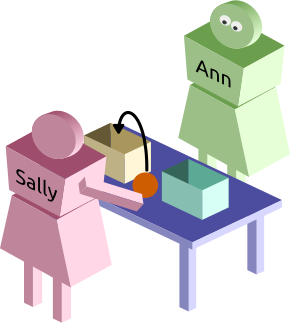
\includegraphics[scale=0.4]{typology/sally_ann1.pdf}
        } \hspace{15pt} %
        \subfigure[She goes away.]{
            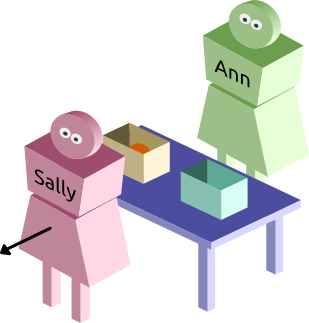
\includegraphics[scale=0.4]{typology/sally_ann2.pdf}
        } \\
        \subfigure[Ann moves the ball.]{
            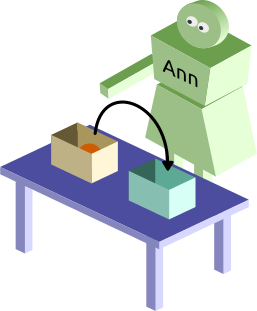
\includegraphics[scale=0.4]{typology/sally_ann3.pdf}
        } \hspace{15pt} %
        \subfigure[Where will Sally look for the ball?]{
            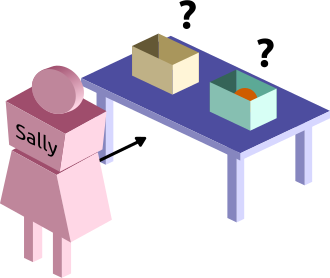
\includegraphics[scale=0.4]{typology/sally_ann4.pdf}
            \label{fig|sally-ann-final}
        }
        \caption{The standard ``Sally and Ann'' false-beliefs experiment, taken
        from~\cite{Leslie2000}.}

        \label{fig|sally-ann}
\end{figure}

Scassellati~\cite{Scassellati2002} is amongst the researcher having studied
theory of mind for robots.



\subsubsection{Introspection: Who am I? What can I do?}
\label{sect|introspection}

\paragraph{Introspection}

Introspection is the ability to self-describe: what are my capabilities, what
is my state (performing some action, idling, etc.), what are my beliefs, what
are my intentions and my plans?

Introspection must be distinguished from meta-cognition: While introspection
may require meta-cognition (for instance to be able to expose its internal
knowledge), it is not always mandatory. The current state of the robot can be
represented as a simple instantiation of a specific category (for instance, if
the robot give an object to the human, this state could be represented with the
triples \setstmt{robot performs action1,action1 isA Give}.

\paragraph{Modelling of the robot capabilities}

A particularly important aspect of introspection relates to the description of
its own capabilities: which sensors/actuators/computation services exist and
are currently available ?  While at a first level, these descriptions can be
static (\eg the robot has one laser scanner and two arms), at more advanced
levels, the description is updated and reflect the current (and possibly past
and future) state of the robot. Note that these description may also involve
geometric descriptions (a kinematic chain, the pose of a device, etc.) that may
be deported outside of the main knowledge base. Efforts trying to formalize,
maintain and expose the capabilities and state of a robot are not new (and
ground themselves in work and techniques for self-descriptive remote procedure
calls in computing science), but take a renewed importance with applications
for high-level multi-robot cooperation. Recent works in that direction
include~\cite{Kunze2011}.

\subsubsection{Memory}
\label{sect|memory}

Memory has been studied at length in the cognitive psychology and
neuropsychology communities: Atkinson and Shiffrin~\cite{Atkinson1968}
introduce the idea of \emph{short-term} and \emph{long-term} memory,
Anderson~\cite{Anderson1976} splits memory into \emph{declarative} (explicit)
and \emph{procedural} (implicit) memories, Tulving~\cite{Tulving1985} organizes
the concepts of \emph{procedural}, \emph{semantic} and \emph{episodic} memories
into a hierarchy. Short-term memory is refined with the concept of
\emph{working memory} by Baddeley~\cite{Baddeley2010}
(Figure~\ref{fig|memory_models}).

\begin{figure}
    \centering
    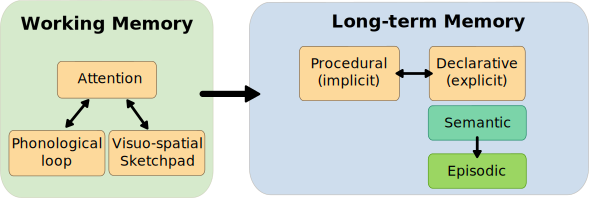
\includegraphics[width=0.6\columnwidth]{typology/memory_models.pdf}
    \caption{Overview of the main types of memories}
    \label{fig|memory_models}
\end{figure}

It worth emphasising that if memory is commonly associated to the process of
forgetting facts after a variable amount of \emph{time}, it actually covers
more mechanisms that are relevant to robotics, like selective remembering
triggered by a specific context or reinforcement learning.

Most knowledge representation systems offers some kind of memory as a pool of
facts that are not forgotten by the robot until it is halted (this memory is
often referred as a \emph{working memory}, but with a meaning unrelated to
Baddeley's definition). Some systems may propose persistent storages that allow
the robot knowledge to grow over time, while other may offer a larger range of
memory categories, like short term memory (that lasts for a couple of seconds)
or episodic memory (that allows the robot to selectively remember facts
associated to specific events).

In the larger field of cognitive architectures, the {\sc Soar}
architecture~\cite{Lehman2006} is one of those that tries to reproduce a
human-like memory organization.

%%%%%%%%%%
\subsection{Reasoning Techniques}
\label{sect|reasoning}

\begin{scriptsize}
\begin{center}
\begin{tikzpicture}[taxonomy]
    \node [taxon] {\bf C. Reasoning}
            child {node [taxon] {{\bf C.10}. Learning}}
            child {node [taxon] {{\bf C.9}. Naive physics}}
            child {node [taxon] {{\bf C.8}. Planning}}
            child {node [taxon] {{\bf C.7}. Prediction and explanation}}
            child {node [taxon] {{\bf C.6}. Presupposition}}
            child {node [taxon] {{\bf C.5}. Non-monotonicity}}
            child {node [taxon] {{\bf C.4}. Uncertainty}}
            child {node [taxon] {{\bf C.3}. Lazy evaluation}}
            child {node [taxon] {{\bf C.2}. Instantiation and structural alteration}}
            child {node [taxon] {{\bf C.1}. Standard reasoning}};
\end{tikzpicture}
\end{center}
\end{scriptsize}


\subsubsection{Standard reasoning techniques}
\label{sect|std-reasoning}

We call \emph{standard reasoning techniques} techniques based on logical
inference, using resolution algorithms like \emph{forward chaining},
\emph{backward chaining} or \emph{semantic tableaux}.

Main reasoning problems include \emph{concept satisfiability},
\emph{consistency checking} and \emph{instance checking}.

Concept satisfiability verifies if it is possible to find a non-empty
\emph{interpretation} of a concept (or an expression defining a concept) in the
knowledge model. For instance, the formula \concept{Plant} $\land$
\concept{isRed}, which defines the concept of red plants, is satisfiable in a
model \concept{KB} iff $\exists a, $ \concept{Plant}$(a) \land$
\concept{isRed}$(a)$, \ie if we can find at least one red plant $a$ in our
model.

Checking the consistency of a model is equivalent to checking the
satisfiability of each of the concept defined in the knowledge model.

Instance checking consists in verifying that an individual $a$ is an
interpretation of a concept (or concept expression) $C$ in the knowledge model.
A typical example would be that we are provided with an instance
\concept{object1} and we want to know if this object is a kind of
\concept{Bottle} or \concept{Glass}.

Inferences can also be drawn from other constructs, whose availability depends
on the representation language. OWL, for instance, has constructs for:

\begin{itemize}
    \item class subsumption (to represent inheritance relations)

    \item reasoning on roles properties, including:
        \begin{itemize}
        \item entailments based on roles domain and range (for instance, if the
        domain of the role \concept{thinksOf} is known to be
        \concept{ThinkingAgent}, then \concept{thinksOf}$(a, b) \to
        $\concept{ThinkingAgent}$(a)$),

        \item universal, existential and cardinality constraints,

        \item several second-order predicates (inverse, symmetry, transitivity, etc.)

        \end{itemize}

    \item \emph{class restrictions} like: \par 
    \footnotesize 
    \concept{Bottle} $\equiv$ \concept{Artifact} {\bf that} (\concept{hasShape}
    {\bf value} \concept{cylinderShape})
    \normalsize

    \item set operations like: \par 
    \footnotesize 
    \concept{Color} $\equiv \bigcup$ (\concept{blue}, \concept{green},
    \concept{orange}, \concept{black}, \ldots) 
    \normalsize

\end{itemize}

\paragraph{Rule Languages} As mentioned earlier, knowledge models based on
description logics can be extended through rule languages (typically for OWL,
the SWRL language).

An intersection of properties is an example of expression that can only be
represented with rules. For instance:

\footnotesize
\concept{looksAt(?agt, ?obj)} $\land$ \concept{pointsAt(?agt,?obj)}
$\Rightarrow$ \concept{focusesOn(?agt, ?obj)}
\normalsize

\subsubsection{Dynamic Instantiation and Alteration of the Knowledge Structure}

The content of a knowledge base is often conveniently divided into a
\emph{structural part} that defines the conceptualisation of a domain in term
of vocabulary and relations between the concepts, and an \emph{instantiation} of
this structure into concrete entities.

The terms TBox and ABox are commonly found to describe this two different types
of statements in ontologies: TBox statements describe a system structure (made,
for example, of a set of classes and properties) whereas the ABox contains
TBox-compliant statements that are asserted in this structure.

Knowledge representation systems allow to modify the ABox, which can be
considered as the dynamic part of the knowledge base. Alteration of the ABox
include the addition or retraction of relations between existing instances,
and the addition or removal of instances. We call the later \emph{dynamic
instantiation}: the capability for a system to create new instances at
run-time. The term dynamic instantiation applies primarily to concrete entities
(typically, a new object is discovered by the robot, a symbolic instance is
created for it), but may also apply to abstract entities (like an instance of
action, of a feeling, etc.).

The knowledge representation system may also allow to alter the TBox. This
requires the underlying reasoning systems to be able to dynamically take into
account structural changes in the knowledge base.

Example of TBox alteration include modification of the taxonomy (like addition
or retraction of a \concept{subClassOf} relation), changes to the asserted
domain or range of a predicate, addition or retraction of rules.

Supporting TBox alteration has notable consequences on the learning
capabilities of the system: teaching general facts (\ie, facts at the level of
whole categories) like ``cars go on roads'' to a robot requires an alteration
of the TBox.

\subsubsection{Lazy evaluation}
\label{sect|lazy-evaluation}

\emph{Lazy evaluation} describes the ability for a KRS to delay active
knowledge acquisition or reasoning operations until the value is actually
needed.

For instance, a system that computes the symbolic relative placement of two
objects only when this fact is required to answer a query would be said to
adopt a lazy evaluation strategy, whereas a system that computes {\it a priori}
such relations (and by consequence, carries out such computation for possibly
all known objects) would be said to use a \emph{strict evaluation} policy.

Lazy evaluation has an immediate impact on efficiency and scalability of the
system, and some problems may even be only tractable with a lazy evaluation
strategy (the relative placements of object is an example of combinatory
explosion in strict evaluation approaches, although this issue could be
mitigated in real use-cases by heuristics that would select a subset of objects
to evaluate).

One downside is that the knowledge base never contains explicitly the complete
set of beliefs of the robot. This limits for instance the ability for the robot
to react to logical conditions that involve facts that are lazily evaluated
(``trigger a callback when object A is behind object B'' would not be triggered
with a purely lazy evaluation strategy for spatial relations).

%\subsubsection{Reasoning with uncertainty}

\subsubsection{(Non) Monotonic Reasoning}

\emph{Monotonic reasoning} means that addition of new assertions to a knowledge base
can only extend the set of assertions that can be inferred, while a
\emph{non-monotonic} reasoning scheme may lead to retraction of facts.
McCarthy coined a famous example to illustrate the need of non-monotonic reasoning:

\begin{quotation}
Consider putting an axiom in a common sense database asserting that birds can
fly. Clearly the axiom must be qualified in some way since penguins, dead birds
and birds whose feet are encased in concrete can't fly. A careful construction
of the axiom might succeed in including the exceptions of penguins and dead
birds, but clearly we can think up as many additional exceptions like birds
with their feet encased in concrete as we like. Formalized non-monotonic
reasoning provides a way of saying that a bird can fly unless there
is an abnormal circumstance and reasoning that only the abnormal circumstances
whose existence follows from the facts being taken into account will be
considered.
\end{quotation}

An important application of non-monotonic reasoning is the representation of
change: for example, to make a brownie, one needs to crack eggs and mix them to the chocolate.
The eggs disappear and are replaced by a dough:

\concept{Egg}$(a) \land $ \concept{Chocolate} $(b) \land $
\concept{MakeDough}$(a, b, c) \to \lnot $ \concept{Egg}$(a) \land \lnot $
\concept{Chocolate}$(b) \land $ \concept{Dough}$(c)$

The insertion of the proposition \concept{MakeDough}$(a, b, c)$ leads to
retraction of other facts. This rule requires non-monotonic reasoning to be
applied.

\emph{Default logic} is one of the formal logic that account for representing
general truth and exceptions to it (for instance, \emph{tomatoes are red, in
general}). However, due to computational complexity of these model (most of
inferences in default logic are known to be $NP$-complete problem), classical
logics and most of the existing reasoners do not allow non-monotonic reasoning.
For instance, the SWRL rule language, usually associated to the OWL-DL ontology
language, do not allow non-monotonic reasoning (only so-called DL-safe rules
are allowed).

\fxfatal{Make clear 'who does not allow non-monotonic-reasoning': logics? rule
languages? reasoner?}

One important exception is the \emph{negation as failure} inference rule, as
implemented by {\sc Prolog} for instance, that allows for non-monotonicity
within the closed world assumption.

\fxfatal{Give here an example of non-monotonic reasoning with Prolog}
\fxwarning{Do we mention here Answer Set Programming?}

A monotonic system does not theoretically allow for knowledge retraction,
which is an important issue in the robotic context where the world model is
likely to be often altered.  However it is a practical issue only if the
reasoning process is \emph{continuous} during the whole robot's activity
lifespan. It is often possible to stop the reasoner, alter the knowledge, and
restart the inference process on a new domain.
\fxfatal{Rephrase to emphasize that when new evidences appear, it is anyway often a
good idea to restart the reasoner.}

\fxfatal{Mention that the 'change of world' issue can also be dealt with appropriate
time representation.}
\fxfatal{Mention that probabilistic reasoning lead to implicit non-monotonic reasoning}


\subsubsection{Presupposition Accommodation}
\label{sect|presupposition-accommodation}

\emph{Presupposition accommodation}~\cite{VonFintel2008} is the ability for a
system to automatically create a context allowing to make sense of a
proposition.

Applied to robotics, we can imagine a human telling a robot ``Please get me the
bottle that is behind you''. If the robot has not yet see what is behind it, it
needs to assume (and represents in its knowledge model) that a undefined bottle
can be found somewhere in the half of space behind it.

A knowledge representation system able to cope with presupposition
accommodation would be able to take into account this (usually under-defined)
information that is not grounded into perception for later inferences.

This ability to imagine a physically state of the world that is not actually
perceived can be seen as the converse of the grounding ability.

Note also that presupposition accommodation implies a bidirectional link of the
symbolic knowledge model with a geometric (or physical) model of the
environment.

\subsubsection{Prediction, projection, explanation}
\label{sect|prediction-projection}

Levesque~\cite{Levesque2008} distinguishes two main tasks related to reasoning
on actions and consequences of actions, the \emph{projection task} and the
\emph{legality task}.

We call \emph{diagnosis} the converse of the projection task: the ability to
track back the origin of a decision...\fxwarning{To be completed, also with
explanation}.

\begin{scriptsize}
\begin{center}
\begin{tikzpicture}[taxonomy]
    \node [taxon] {\bf C.6 Prediction and Explaination}
            child {node [taxon] {{\bf D.4} Explaination}}
            child {node [taxon] {{\bf D.3} Diagnosis}}
            child {node [taxon] {{\bf D.2} Legality}}
            child {node [taxon] {{\bf D.1} Projection}};
\end{tikzpicture}
\end{center}
\end{scriptsize}


\paragraph{Projection task}: determining whether or not some condition while
hold after a sequence of actions. The projection task is a typical
non-monotonic reasoning task, since at each step, the system must add but also
retract beliefs, as defined in the tasks post-conditions.

\paragraph{Legality task}: determining whether a sequence of action can be
performed starting in some initial state.

\paragraph{Diagnosis}: this corresponds to the ability to rewind on past events
in case of failure to provide possible explanation. This can be seen as the
temporal reverse of the projection task. Because of their modelling of
situations as an history of actions, derivatives of the GOLOG logic programming
languages are a good example of the diagnosis task integrated to the knowledge
representation system~\cite{Gspandl2011}.

\paragraph{Explanation} Diagnosis is also linked to the \emph{explanation} or
\emph{justification} capabilities that may be offered by the knowledge
representation system. The explanation of an entailment is the sequence (or
set of sequences if several are possible) of reasoning steps that allow to
reach a conclusion. An explanation can also conversely explain why a statement leads to a
contradiction.

The following example shows an explanation for an inconsistency in a particular
knowledge base: by adding the statement \stmt{robot1 belongsTo human1}, we
observe that an inconsistency is triggered. The reasoner provides the four
following observations to explain the inconsistency:

\begin{quote}
\scriptsize
\begin{enumerate}
    \item \concept{robot1} {\bf Type} \concept{belongsTo} {\bf some} \concept{Thing}
    \item \concept{belongsTo} {\bf Domain} \concept{Artifact}
    \item \concept{robot1} {\bf Type} \concept{Agent}
    \item {\bf DisjointClasses:} \concept{Agent}, \concept{Artifact}
\end{enumerate}
\normalsize
\end{quote}

This explanation directly portrays the underlying structure of the knowledge
model: we can understand that a robot is modelled here as an agent, that agents
and artifacts are disjoint classes and that only artifacts can belong to
someone, hence the inconsistency. A KRS may provide mechanisms to expose this
kind of analysis, either automatically when inconsistencies occur, or on
demand.

Explanation of contradictions plays a particular role for robots: from a
cognitive point of view, a logical inconsistency (\ie, a contradiction) can be
viewed as a \emph{cognitive conflict} or \emph{cognitive dissonance} (\ie, two
incompatible models of the world that must be dealt with). Being able to expose
and explain such cognitive conflicts eases the control of the behaviour of the
robot in unexpected semantic situations, and forms a first step towards an
adequate reaction.

Cognitive dissonance is also identified by developmental psychologists like
Piaget as a motivation factor for a child to progress through the various
stages of its cognitive development. This has been also studied in
robotics~\cite{Oudeyer2007}.


The cognitive capability of \emph{justification} is also intimately linked to
the meta-cognition capability and participates to the overall \emph{cognitive
observability} of the system.

\subsubsection{Task Planning}
\label{sect|planning}

Symbolic task planning is the ability for a robot to select a sequence of
actions in order to reach a given final state. This capability is closely
related to the previously mentioned projection and legality tasks: for a robot
to plan, it must be able to build hypothetical states of the world that would
follow from the successive application of actions (prediction task), and at
each step, select possible, legal actions based on their pre-conditions
(legality task). As already mentioned, these tasks are highly non-monotonic.


Symbolic task planning in general is a large research
field~\cite{Russell2009planning}. The so-called Classical Planning Problem,
first, is characterised by a unique known initial state, durationless
deterministic actions which can be taken only one at a time, and a single
agent. STRIPS and PDDL are amongst the commonly used languages for representing
such planning problems.

Planning with nondeterministic durationless actions with probabilities can be
represented as discrete-time \emph{Markov decision processes} (MDP), and when
full observability is replaced by partial observability, we deal with
\emph{partially observable Markov decision process} (POMDP).

\emph{Hierarchical Task Networks} (HTN) are another common formalism for
planning problems, where an initial set of tasks (\emph{High Level Tasks}, HLA)
is decomposed into either primitive actions or a new set of subtasks.

From the observation that the core reasoning techniques (back and forward
chaining) are shared between planners and reasoners used in knowledge
representation systems, task planning can be considered within the KRS.

Since McCarthy's \emph{Situation Calculus} in 1963, numerous knowledge
representation formalisms dedicated to representation and reasoning about
actions and situation have emerged: besides situation calculus, \emph{fluent
calculus} and \emph{event calculus} are the main ones.
Thielscher~\cite{Thielscher2011} recently proposed a unification of these
approach in a new \emph{action calculus}.

The GOLOG~\cite{Levesque1997} language and its derivatives (like {\sc
ReadyLOG}~\cite{Ferrein2008} and {\sc IndiLOG}~\ref{Gspandl2011}) propose
implementations of the situation calculus focused on robotic applications.


It is however also common to rely on external components dedicated to symbolic task
planning (in particular because of the non-monotonicity requirements) with a
tight link to the KRS for domain retrieval and/or resulting plan storage.

Finally, in the context of interaction between several agents, the management
of \emph{joint intentions} and \emph{joint goals}~\cite{Tomasello2005,
Bratman2009} are additional aspects that have to be represented and
appropriately handled by the planning subsystem.

%An extensive report on task modeling in OWL ontologies in appendix

\subsubsection{Physics-based reasoning}
\label{sect|physics}

As embodied entities, robots have to interact with physical entities.
\emph{Naive physics reasoning} covers all the everyday reasoning the humans
unconsciously perform, like taking into account gravity (``if I drop a ball, it
falls down'') or common physical properties of objects (``a glass may break if
dropped'', etc.). Many of the interactions with our everyday environments are
ruled by such laws that are difficult to exhaustively encode.

Some systems \cite{Kunze2011a} rely on external dedicated physics engine to
compute symbolic facts from on-demand physics simulation. This requires a tight
integration between the symbolic model and a geometric model that carries the
geometries and physical properties of objects.

\subsubsection{Learning}
\label{sect|learning}

\fxfatal{Learning section to write}

%%%%%%%%%%%%%%%%%
\subsection{Acquiring Knowledge}

\begin{scriptsize}
\begin{center}
\begin{tikzpicture}[taxonomy]
    \node [taxon] {\bf D. Acquisition}
            child {node [taxon] {{\bf D.3} Motivation}}
            child {node [taxon] {{\bf D.2} Grounding}}
            child {node [taxon] {{\bf D.1} Acquisition and fusion}};
\end{tikzpicture}
\end{center}
\end{scriptsize}

\subsubsection{Knowledge acquisition and modalities fusion}
\label{sect|knowledge-acquisition}

In our context, \emph{acquiring knowledge} means to build new logical
statements from data sources and to anchor them into the existing knowledge. We
consider three possible sources of data: proprioceptive/exteroceptive sensing,
interaction with other agents, humans or robots, and remote knowledge bases.
The acquisition process has generally two steps: the information acquisition by
itself, and the \emph{transformation} of the information into knowledge,
\emph{aligned} with the robot existing model (following our terminology for
information and knowledge, as discussed at the beginning of the chapter).

It must be observed that knowledge acquisition is generally not done directly
in the knowledge representation system. External components (often aggregated
into knowledge acquisition \emph{pipelines}) are usually required to convert
percepts into symbolic facts and to ground them.

While we do not review in this article all these systems, the whole process of
knowledge acquisition is central in cognitive robotic architecture and the
design of knowledge representation systems can influence or be influenced by
the approach to knowledge acquisition.

In particular, complex robotic systems often require multi-modal perception
capabilities (for instance, a robot can only interpret an utterance like ``this
is a plate'' if it is able to understand gestures, understand natural language
and merge them in a timely manner). Multi-modal interpretation can take place
at various levels, but in many cases (especially if the modalities are of very
different natures, like in the example above) merging will require
symbolic-level reasoning. The KRS has a direct impact on the feasibility and
ease of such operations.

Let review shortly the three sub-categories of knowledge acquisition.

\begin{scriptsize}
\begin{center}
\begin{tikzpicture}[taxonomy]
    \node [taxon] {\bf D.1 Acquisition and fusion}
            child {node [taxon] {{\bf D.1.3} Linked Resources}}
            child {node [taxon] {{\bf D.1.2} Interaction}}
            child {node [taxon] {{\bf D.1.1} Sensing}};
\end{tikzpicture}
\end{center}
\end{scriptsize}

\paragraph{Sensing}

From the point of view of knowledge representation, the sensing capability can
be split into proprioceptive sensing (\ie, sensing of the robot own internal
state) and exteroceptive sensing (sensing of the robot environment). The
(physical) introspection capabilities of the robot relies on the former.

\fxwarning{What to say here?}

\paragraph{Interaction}

Interaction with other intelligent agents (humans or robots) is another
important source of knowledge acquisition. It relies obviously on some form of
sensing (from speech recognition to gesture recognition) but we distinguish it
from the previous section because \emph{interaction} implies a form of
communication. Communication is associated to specific functions
(as shown on Jakobson's diagram, figure~\ref{fig|jakobson_communication_model},
page~\pageref{fig|jakobson_communication_model}), and in particular, it implies
a shared context (usually implicit) between interactors.

We distinguish between two main interaction channels: verbal and deictic.

\begin{scriptsize}
\begin{center}
\begin{tikzpicture}[taxonomy]
    \node [taxon] {\bf D.1.2 Interaction}
            child {node [taxon] {{\bf D.1.2.2} Deictic Interaction}}
            child {node [taxon] {{\bf D.1.2.1} Verbal Interaction}};
\end{tikzpicture}
\end{center}
\end{scriptsize}

\label{sect|nlp}

The field of verbal interaction processing for robots spans from pattern-based,
constrained sentences recognition to natural, bidirectional, unconstrained
verbal communication. A large literature corpus exists on Natural Language
Processing (NLP) which is presented at section~\ref{sect|dialogs-related-work},
page~\pageref{sect|dialogs-related-work}.

NLP is an established research field by itself, and while the robotic community
is still lagging behind on many theoretical aspects, it brings one important
aspect: the embodiment. Because the interactors, both the robot and the human,
are establishing a communication within a shared physical context, the verbal
communication channel is complemented by deictic channels, back channels and
possibly shared physical experiences: a human can show something to a robot,
saying ``Give me this''. This is not possible for a virtual agent.

Several of the knowledge representation systems we present have developed
specific built-in mechanisms or extensions to parse, ground and possibly
rebuild natural language.

Deictic (used in the literal meaning of ``display, demonstration, reference'')
interaction is also an established field of research in human-robot
interaction. Common deictic forms of communication~\cite{Li2012} include
attentional focus (via face and gaze tracking) and joint attention, pointing,
emotional expressions (based on face expressions, postures, emotional
gestures).

Like other knowledge acquisition modalities, the recognition and interpretation
of deictic communication is rarely directly included in a KRS, but, as
previously mentioned, the symbolic representation of such communication acts is
relevant and important to achieve successful multi-modal interactions.

\paragraph{Linked Knowledge Resources}
\label{sect|lod}

Robots, and in particular service robots, have usually an access (with possibly
security-related constraints) to the World Wide Web and remote knowledge stores.

The current shift towards the Semantic Web (\ie structured, annotated data that
are easily machine-processable) makes increasingly easy to have robots to reuse
autonomously this knowledge. The DBPedia project, for instance, illustrates
well the tendency: it provides an automatically generated RDF version of the
Wikipedia encyclopedia.

In its current state, the relevance of the DBPedia project in our context is
however limited: the triples that are extracted are mostly ``mechanical'' (like
the categories of a term, or factual informations extracted from Wikipedia's
InfoBox), and the vast majority of the knowledge actually contained in the
encyclopedia pages remains out of reach of automated parsers. Efforts in that
direction however exist~\cite{Nyga2009, Fader2011}.

Another notable project that seeks at providing large amount of
machine-friendly common-sense knowledge is the MIT's OpenMind
project~\cite{Singh2002}. The project is designed to let the general public
easily add common-sense statements in semi-controlled natural language, which is
then processed to a publicly available ontology.

Another approach that is easier at short-term to let robots remotely access
knowledge repositories consists is building robot-specific shared repositories,
with declarative and/or procedural (\ie, plan library) knowledge. The
RoboEarth~\cite{Waibel2011} project is an example of such an effort.

\subsubsection{Grounding/anchoring strategies}
\label{sect|grounding}

\emph{Grounding} (also called \emph{anchoring} when specifically referring to the
building of links between \emph{percepts} and \emph{physical
objects}~\cite{Coradeschi2003}) is the task consisting in building and
maintaining a bi-directional link between sub-symbolic representations (sensors
data, low-level actuation) and symbolic representations that can be
manipulated and reasoned about~\cite{Harnad1990}.

Being embodied entities with interaction with other embodied entities as a
fundamental requirement, robots and robotic is deeply concerned by the
grounding issue.

Being actually implemented on real service robots, all the symbolic knowledge
representation systems that we review in this study have some kind of grounding
process. Numerous approaches exist, like amodal
\emph{proxies}~\cite{Jacobsson2008}, grounded amodal
representations~\cite{Alami2011, Mavridis2006}, semantic maps
(Figure~\ref{fig|semanticmap}, \cite{Nuechter2008, Galindo2008,Blodow2011}) or
affordance-based planing and object classification~\cite{Lorken2008,
Varadarajan2011}.

\fxwarning{Un peu court!}

\begin{figure}
    \centering
    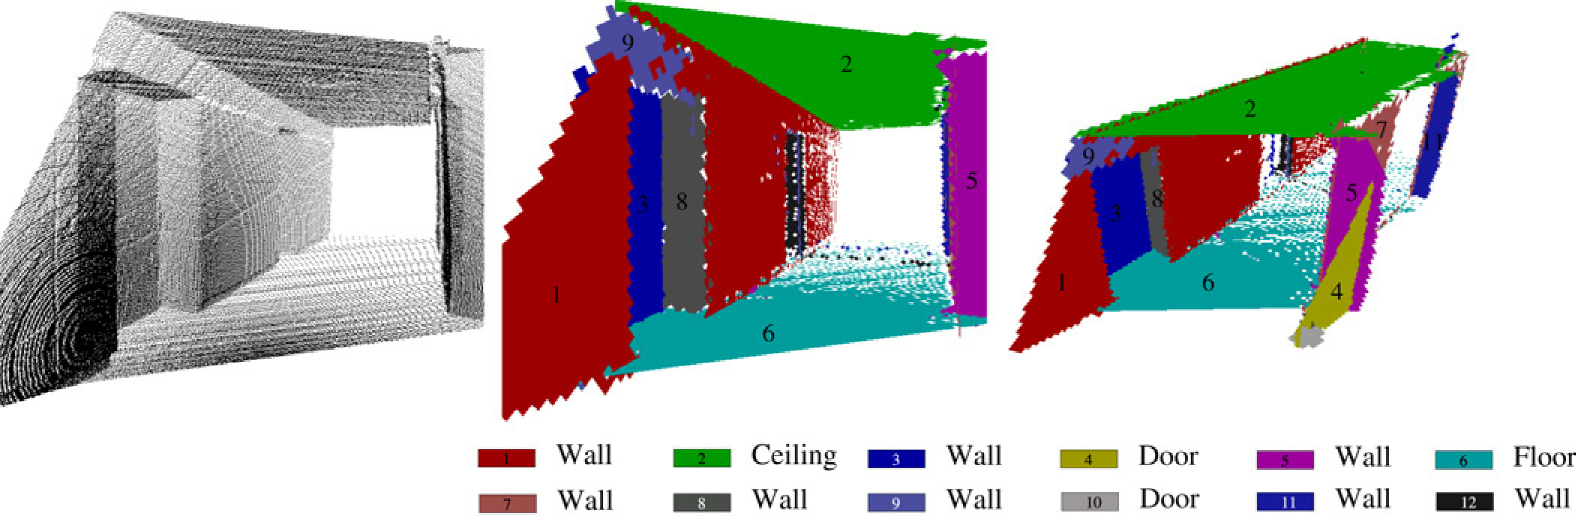
\includegraphics[width=0.9\columnwidth]{typology/semanticmaps_hertzberg.png}
    \caption{Example of a semantic map, taken from~\cite{Nuechter2008}.}
    \label{fig|semanticmap}
\end{figure}

\subsubsection{Intrinsic Motivation and Curiosity}

The reasons for a robot to acquire knowledge are diverse, and usually external
to the robot itself. It is often driven by the requirements of tasks that the
robot has to execute. In this case, motivations are managed by the execution
controller and are mostly invisible to the knowledge representation system.

However, motivation can also be intrinsic, driven by the internal state of the
robot's beliefs, without external pressure or reward. In this case, the \fxwarning{to be completed}

In the context of robotics, Oudeyer notes however that \emph{the information that is
compared \emph{[to compute a level of motivation]} has to be understood in an
information theoretic perspective, in which what is considered is the intrinsic
mathematical structure of the values of stimuli, independently of their
meaning.}~\cite{Oudeyer2007}.

Psychological grounds of motivation are summarized in~\cite{Oudeyer2007} while
the main approaches to computational motivation, divided into knowledge based
models, competence based models and morphological models, are surveyed
in~\cite{Oudeyer2008}.

%%%%%%%%%%%%%%%%%
\subsection{Practical Integration in Robotic Architectures}
\label{sect|integration-robot}

\begin{scriptsize}
\begin{center}
\begin{tikzpicture}[taxonomy]
    \node [taxon] {\bf E. Integration}
            child {node [taxon] {{\bf E.4} Performances}}
            child {node [taxon] {{\bf E.3} Monitoring}}
            child {node [taxon] {{\bf E.2} Executive layers}}
            child {node [taxon] {{\bf E.1} Sensori-motor}};
\end{tikzpicture}
\end{center}
\end{scriptsize}


Knowledge representation systems do not mean anything to robots if they are
considered in isolation. This section proposes categories of features related
to the integration of the KRS into a larger software architecture that includes
perception routines, decision-making processes and actuation control.

We also mention some practical aspects of a real-world system, like
performances and monitoring tools that come along with the KRS.

\subsubsection{Integration with sensori-motor layers}
\label{sect|integration-sensorimotor}

We have previously discussed (section~\ref{sect|grounding}) the principles of
the grounding process that aims at establishing and maintaining a connection
between percepts (and to a lesser extend, low-level actions) and symbols.

While every real-world cognitive robot need some kind of grounding, the actual
implementations lead to very different information flows.

The systems can be roughly split into two classes: \emph{passive} knowledge
repositories that process symbolic facts produced by lower-level sensori-motor
layers (\emph{push} flow); \emph{active} knowledge managers that directly query
(possibly by polling or on-demand) low-level layers.

This macroscopic distinction is however mostly a matter of defining the
frontiers of the KRS: some systems like KnowRob~\cite{Tenorth2009a} encompass
geometric reasoning layers that would be considered as external by other
systems like ORO~\cite{Lemaignan2010} that focus on the symbolic fact storage
and rely on a ecosystem of independent modules to provide and consume symbolic
knowledge.

\fxwarning{Some archi with the ability to ``listen'' to the robot internal
structures -> which ones?}

Other systems do not fit either in such a partition between active and passive
systems because they do not stand as independent modules but exist as diffuse,
\emph{ubiquitous} knowledge manipulation system (case of the CAST knowledge
model~\cite{Jacobsson2008}), for instance because they are primarily
language~\cite{Ferrein2008, Sabri2011}.

\subsubsection{Integration with executive layers}
\label{sect|integration-executive-layers}

Conversely, the knowledge management module need a tight integration with the
decision-making processes. As for the integration with sensori-motor
layers, the borders of the KRS can be fuzzy and vary from one architecture to
another: many consider symbolic task planning as an integral role of the KRS,
while other have dedicated extensions for planning, some integrate learning as
an on-the-flight process that is part of the KRS, others as an independent
deliberative process, etc.

The actual integration techniques vary also widely, from language extensions
(like the integration of CRAM~\cite{Beetz2010} with KnowRob) and client-server
architectures, to event-driven models (SHARY and ORO~\cite{Alami2011}). Choices
at this level have notable consequences on the whole design of the upper
control architecture of the robot, in particular regarding its modularity and
the ease of addition of new components.

\subsubsection{Monitoring and debugging}
\label{sect|debugging}

It is common to have knowledge representation systems at the heart of a
cognitive robotic architecture, and therefore KRS are easily ``buried'' in the
system.

At the same time, the symbolic model often provides a valuable synthetic view
on the whole state of the robot, furthermore easily understandable by the human
developer (the fact \stmt{human1 isSitting true} is easier to interpret than
the suite of relative coordinates of each joints of the human skeleton, as
provided by the human tracker, for instance).

Tools to trace and visualise at run-time the evolution of the knowledge
structure and contents may be available with the KRS, as well as
post-processing tools that run on the trace to analyze {\it a posteriori} the
cognitive behaviour of the robot.

\subsubsection{Evaluation of performances}
\label{sect|performances}

Benchmarks of symbolic systems for robots are hard to conduct for several
reasons: identifying good metrics for robotic experiments in general is
difficult because of the complex interactions between tenth of modules running
in parallel, and isolating one specific component is difficult.  Also,
knowledge representation systems are often tightly coupled to the other
modules. To quote Langley~\cite{Langley2006}:

\begin{quote}
The conventional wisdom of software engineering is that one should
develop independent modules that have minimal interaction. In contrast, a
cognitive architecture offers a \emph{unified} theory of cognition with tightly
interleaved modules that support synergistic effects.
\end{quote}

The lack of standard API for knowledge services makes it also hard to switch
between KRS to compare them.

Finally, because service robots are designed to act in rich, dynamic
environments, possibly with humans, building repeatable experiments is
challenging, and quantitative measurements are often not the right
metric~\cite{Langley2006}.

We will however present here some quantitative metrics (related to scalability,
for instance), followed by qualitative evaluation approaches, grouped under the
term \emph{Cognitive Performances}.

\begin{scriptsize}
\begin{center}
\begin{tikzpicture}[taxonomy]
    \node [taxon] {\bf E.4 Performance \\Evaluation}
            child {node [taxon] {{\bf E.4.2} Cognitive Performances}}
            child {node [taxon] {{\bf E.4.1} Raw Performances}};
 \end{tikzpicture}
\end{center}
\end{scriptsize}


\paragraph{Raw Performances} The \emph{raw performance} is evaluated on
quantitative benchmarks. The main metric is the \emph{scalability}
$\mathcal{S}^{KRS}$ of the system with the size of the knowledge base
$\sigma=|\Delta^{\mathcal{I}}|$  (in term of atoms or statements).

We call \emph{relaxation time} $\mathcal{R}^{\mathcal{M}}$ the (averaged) time
required by the system after a model modification of type $\mathcal{M}$ before
being available for further interaction, and \emph{query time}
$\mathcal{Q}^{\mathcal{M}'}$ the (averaged) time to execute a query of
complexity $\mathcal{C}$ on the KRS. The type $\mathcal{M}$ of model
alteration is either an ABox modification (addition/removal of an instance) or
a TBox alteration (addition/removal of a class, a class restriction or a rule).
Query complexity $\mathcal{C}$ is...\fxwarning{find references}.

\emph{Temporal scalability} is defined in term of the nature of the function
$f^{\mathcal{M}, \mathcal{C}}(\sigma) = \mathcal{R}^{\mathcal{M}}(\sigma) +
\mathcal{Q}^{\mathcal{C}}(\sigma)$ (\ie the relation of the relaxation time
and query time to the knowledge base size). \emph{Space scalability} is the
relation of memory consumption to the size $\sigma$. The scalability is tightly
coupled to the expressiveness of the underlying knowledge model, which need to
be known for the scalability measurement to be meaningful.

Because of coupling and repeatability issues we have mentioned, raw
performances of KRS are often benchmarked with synthetic datasets (which leads
to another issues: how to assess the meaningfulness of the performance of a
reasoner on an artificial ontology?~\cite{Bail2010}) or ``toy'' experiments
that do not always model the whole complexity of real-world
application~\cite{Chong2009}.

\paragraph{Cognitive Performances} While evaluating the raw performances of
knowledge representation systems in a relevant manner may be difficult, the cognitive
performances of the robot as a whole can be also evaluated.

Langley et al.~\cite{Langley2006} propose five such dimensions of evaluation:
the \emph{generality} of the system (can it adapt easily to new tasks?), the
\emph{rationality} or relevant of the inference/reasoning/decisions the system
take, the \emph{reactivity} and \emph{persistence} that evaluates if the
behaviour of a cognitive system is appropriate under unpredicted changes, the
\emph{improvability} of the system as a function of the knowledge added to it,
and finally, the resulting \emph{autonomy} of the system.

Cognitive performance can also be evaluated with the support of tools developed
in cognitive psychology. Several standard tests (like False-Belief
experiments~\cite{Leslie2000} or the Token test~\cite{DiSimoni1978}) have been
used to judge the cognitive abilities of robots~\cite{Mavridis2006,
Breazeal2006}.
%%%%%%%%%%%%%%%%%%%%%%%%%%
\subsection{Knowledge instantiation}

\begin{scriptsize}
\begin{center}
\begin{tikzpicture}[taxonomy]
    \node [taxon] {\bf F. Knowledge instantiation}
            child {node [taxon] {{\bf F.5} Self-Knowledge}}
            child {node [taxon] {{\bf F.4} Metrics}}
            child {node [taxon] {{\bf F.3} Granularity}}
            child {node [taxon] {{\bf F.2} Common-sense and Alignement}}
            child {node [taxon] {{\bf F.1} Design Strategy}};
 \end{tikzpicture}
\end{center}
\end{scriptsize}

This last branch of our taxonomy looks at the actual \emph{content} of the
knowledge base: the knowledge instantiation. Here, \emph{instantiation} does
not only refer to the instantiation of the knowledge structure (what we have
called the ABox), but also includes the knowledge structure itself (the TBox).

While we have previously mentioned features of knowledge representation system
that enable the robot to fill its knowledge base with content and alter the
knowledge structure, most of the systems also come with a certain amount of
initial knowledge that often includes \emph{common-sense} knowledge (\ie facts
that widely known to humans, and hence often implicit: ``to put a cake in the
oven, one must first open the oven's door'').

The design strategy, the choice to rely on common-sense knowledge or not, the
reuse of standard ontologies, the quantity of {\it a priori} knowledge are many
parameters that lead to different knowledge models.

\fxfatal{Knowledge Instantiation: THIS SECTION IS FAR FROM COMPLETE}

\subsubsection{Design Strategy}
\label{sect|design-strategies}

Ontology engineering has grown into a research field of its own, covering
formalized methodologies for ontology creation, reuse, modularisation, etc.

The creation

Two main approaches are common in the cognitive robotic community:
\emph{top-down} design and \emph{bottom-up}.

\subsubsection{Common-sense and alignment with Standard Upper-ontologies}

At section~\ref{sect|lod} we have presented how remote knowledge bases are a
valuable source of knowledge, including common-sense knowledge, that robot can
extract.

\subsubsection{Granularity}

The knowledge \emph{granularity} qualifies the level of details or refinement
of the knowledge stored.

...

The storage of literal values is a particular case: while knowledge
representation systems have been considered until now mostly as symbolic
systems, they can often represent literal values (in particular, numerical
values) as well.

Depending on the representation language, literal values can be naturally
represented and processed (common case in logic programming language) or not
(storing numerical value, let alone matrices, in OWL is cumbersome).

\subsubsection{Metrics}

Qualitative and quantitative metrics give an insight on the size and
complexity of ontologies.

Table~\ref{table|upper_onto_metrics} gives such metrics for five major
upper-ontologies commonly used in the semantic Web community (taken
from~\cite{Mascardi2007} and the projects' respective websites).

These metrics do not always reflect adequately the \emph{expressive
complexity}, though: in most of these ontologies with a large amount of terms
and assertions, taxonomic relations (\concept{isA}) or technical predicates
(URI, translations, etc.) account for a large part of the assertions, at the
expense of fine semantic relations.

\begin{table}
\begin{center}

\begin{tabular}{llllll}
\toprule
{\bf Project} & {\bf Terms} & {\bf Assertions} \\
\midrule
Cyc & > 300 000 & > 3 000 000 & \\
YAGO & > 10 000 000 & > 120 000 000 \\
SUMO & 20 000 & 60 000 \\
DBPedia (for English) & 1 840 000 & 385 000 000\\
OpenMind Common Sense (for English) & & 1 000 000\\
\bottomrule

\end{tabular}
\end{center}
\caption{Size of the ABox for major upper-ontologies.}
\label{table|upper_onto_metrics}
\end{table}

Other metrics that include the categories of predicates that are used, or the
computed DL expressiveness, can be more significant (some are presented in
table~\ref{table|onto-stats}, page~\pageref{table|onot-stats}).

\subsubsection{Self-Knowledge}

``Self-knowledge'' is the term used in psychology to describe the knowledge
that an individual has, acquires or infers about itself through its
experiences. It answers the question ``What am I like?''.

For a robot to have at its disposal self-knowledge is closely link to the
introspective capability that we have previously mentioned
(section~\ref{sect|introspection})


%%%%%%%%%%%%%%%%%%%%%%%%%%%%%%%%%%%%%%%%%%%%%%%%%%%%%%%%%%%%%%%%%%%%%%%%%%%%%%%%%%%%%%%%%%%
\section{Existing Systems for Knowledge Representation in Service Robotics}
\label{sect|surveyed-systems}


Table \ref{table|surveyed-systems} lists the knowledge representation
systems that we have surveyed.

This section first clarify the inclusion criteria, and then briefly presents
each of them. At chapter~\ref{chapt|evaluation}, we will consider again these
systems, this time as a whole, to build a summary of the fields of knowledge
representation that are adequately (or not) tackled by the existing systems.

\begin{landscape}
\begin{table}\scriptsize
\begin{center}

\begin{tabular}{p{2.2cm}p{1.6cm}p{4cm}lp{2.4cm}p{3.4cm}p{1.5cm}}
\toprule
{\bf Project} & {\bf Category} & {\bf Authors (Institution)} & {\bf Project homepage} & {\bf Programming language} & {\bf Knowledge model/Logical Formalism} & Main reference \\
\midrule
ARMAR/Tapas & Formal & Holzapfel, Waibel \par (Karlsruhe TH) & & & TFS (Typed Feature Structures) & \cite{Holzapfel2008}\\
CAST Proxies & Ubiquitous & Wyatt, Hawes, Jacobsson, Kruijff (Brimingham Univ., DFKI Saarbrücken) & & & Amodal proxies & \cite{Jacobsson2008} \\
GLAIR & Formal & Shapiro, Bona \par (Buffalo Univ.) & & & SNePS & \cite{Shapiro2009} \\
GSM & Structural & Mavridis, Roy \par (MIT MediaLab) & & & & \cite{Mavridis2006} \\
Ke Jia Project & Formal & Chen et al. \par (Univ. of Science and Technology of China) & \url{www.wrighteagle.org/en} & ASP (Answer Set Programming) & ASP & \cite{Chen2010} \\
{\sc KnowRob} & Formal & Tenorth, Beetz \par (TU Munich) & \url{ias.in.tum.de/kb/wiki} & {\sc Prolog} & {\sc Prolog} + OWL-DL &  \cite{Tenorth2009a} \\
NKRL & Language & Zarri et al. \par (Paris Est Créteil Univ.) & & NKRL & & \cite{Sabri2011} \\
%OBOC & KRS & Mendoza & & & & & \cite{Mendoza2005} \\
OUR-K/OMRKF & Formal & Lim, Suh et al. \par (Hanyang Univ.) & \url{incorl.hanyang.ac.kr/xe} & ? & DL + Horn Clauses &  \cite{Lim2011, Suh2007} \\
%ORO & KRS & Lemaignan, Alami \par (LAAS-CNRS) & \url{oro.openrobots.org} & {\sc Java} & OWL-DL ({\sc Jena}) & {\sc Pellet} & \cite{Lemaignan2010} \\
PEIS KR\&R & Formal & Daoutis, Coradeshi, Loutfi, Saffiotti \par (Örebro Univ.) & \url{www.aass.oru.se/~peis} & {\sc C}, {\sc CycL} & CycL (1st and 2nd order logics, modal logics) & \cite{Daoutis2009} \\
%Golog & Language & Levesque (Toronto Univ.) & & {\sc Prolog} & & & \\
% & & Varadarajan, Vincze \par (TU Wien) & & & & & \cite{Varadarajan2011} \\ % -> affordances, but no implementation on a robot
% & & Kaelbling, Lozano-Pérez \par (MIT CSAIL) & & & & & \cite{Kaelbling2011} \\ % -> mostly planning under uncertainty
% & & Hertzberg (Osnabrück Univ.) \\ % -> affordances, semantic mapping
% (based on {\sc KnowRob} & & (JSK) \\

\bottomrule

\end{tabular}
\end{center}

\caption{List of surveyed systems. Categories are \emph{Formal} for systems
that have a formal underlying knowledge representation, \emph{Ubiquitous} for
systems where knowledge is fully distributed, \emph{Language} for languages
used as KRS on robots or \emph{Structural} for KRS where knowledge is
represented as special data structures.}

\label{table|surveyed-systems}
\end{table}
\end{landscape}

\subsection*{Survey Inclusion Criteria}
\label{sect|inclusion-criteria}

Every robotic system has, implicitly or not, some knowledge representation
systems. It may range from a simple state vector to an explicit symbolic
knowledge base.  This survey focuses on the right end of this spectrum:
symbolic systems, suited for abstract reasoning.

Besides, we have decided to restraint the set of systems to those actually
implemented on robots, and used in semantic-rich environments (\ie dynamic,
partially unknown environments with a large range of different entities which
may have interactions). The typical scenario that would involve such robots
is the \emph{Brownie Scenario} already presented at
section~\ref{sect|scenario}: a service robot in a human-friendly environment
like a kitchen.

We have limited ourselves to systems that
\begin{inparaenum} 
    \item  run on \emph{service robot} (that is, robots that interact with 
    objects in a semantic-rich environment primarily designed for humans),
    \item  ground the knowledge in the physical world (physically embedded
    systems able to assess their environment),
    \item  are able to merge different knowledge modalities,
    \item  are able of on-line, dynamic knowledge acquisition and reasoning 
    (\ie not simple static databases).
\end{inparaenum}

These criteria exclude platforms like {\sc DyKnow}~\cite{Heintz2004}
which are focused on data fusion and knowledge grounding at lower levels.

We have also chosen not to include the GOLOG language and its
derivatives~\cite{Levesque1997, Ferrein2008, Gspandl2011} in this survey. While
several implementations on robots, including service robots, do exist, the
focus of this language is on representation and reasoning about actions and
situations, and the link with symbolic, abstract knowledge is not explicit.

While classical cognitive architectures like {\sc Soar}~\cite{Lehman2006} or
{\sc ACT-R} have declarative knowledge modules~\cite{Derbinsky2010} and have
been recently used on service robots (see {\sc ACT-R/E}~\cite{Kennedy2009} for
instance), they are also absent from this survey because we did not find much
references in the literature on knowledge manipulation and representation
applied to robotic scenarii for these architectures.

A comprehensive reference on (bio-inspired) cognitive architectures is also
available from the BICA Society~\ref{BicaCogArch2011}.

\subsection{ARMAR/Tapas}

{\sc Tapas} is the name of the knowledge representation system and dialogue
manager found on the ARMAR~III robot~\cite{Holzapfel2008} for the Karlsruhe
Institute of Technology.

Knowledge in {\sc Tapas} exists as procedural knowledge (plans) and declarative
knowledge. The later is split into \emph{lexical knowledge}, \emph{semantic
knowledge} and a database of identified objects (with their properties). The
\emph{lexical knowledge} contains lexical and grammatical informations about
the objects. The \emph{semantic knowledge} is organized into an ontology
relying on \emph{typed feature structures} (TFS~\cite{Carpenter1992}, a
formalism originating from the computational linguistics community, and a
superset of first-order logic).

{\sc Tapas} has a strong focus on natural language grounding. It proceeds by
generating grammars from properties represented in the ontology to parse and
understand dialogue.

Another focus is put on handling unknown words and objects. {\sc Tapas}
provides routines to recognize unknown entities, and propose and interactive
and iterative verbal process to categorize (including adding new categories)
those new concepts.

\fxwarning{ARMAR: 2 lines on the experiments}

\subsection{CAST Knowledge model}
\label{sect|cast}

CAS (\emph{CoSy Architecture Schema}) Toolkit~\cite{Hawes2007} is a
comprehensive toolkit aimed at building cognitive architectures for robots
through a set of interconnected \emph{SA} (\emph{subarchitectures}). The CAS does not
expose a central knowledge base as seen in other works. It represents instead knowledge as unrooted \emph{proxies}. Those proxies are formally
defined in \cite{Jacobsson2008} as $p= \langle F_p, u_p \rangle$ where $F_p$ is
a set of instantiated features (like $\phi^{Colour}_{red}$) and $u_p$ a
\emph{proxies union} that form an equivalence class corresponding to one
entity.

A union of proxies forms a global amodal representation of an entity, that can
be explicitly shared and manipulated. Being not centralized, the knowledge
model can be qualified of \emph{ubiquitous}. Furthermore, knowledge source in
the CAS architecture is tightly bound to the on-line grounding process (be it
grounded in perception or in dialogue). While nothing seems to prevent it, no
{\it a priori} knowledge (including common-sense knowledge) is used.

Knowledge sharing is ensured by the event mechanism of CAST: modules can
monitor proxies for alteration by other modules. Jacobsson et al. mention how
this can apply to reinforcement learning: the vision module creates a proxy for
an orange object. This proxy get monitored by a learning module. In parallel,
the proxy is bound to an union by the natural language understanding module
that add new a feature like \emph{"this object is a fruit"}. The learning
module is called back, and can add this new information to its model.

In the presented implementation, the CAST knowledge model does no allow for
effectively representing actions or temporal information.\fxfatal{What about
reasoning? can they retrieve for example 'all proxies for colorful objects'?}

\paragraph{Knowledge Acquisition} Several techniques for knowledge acquisition
have been explored within the CAST framework. Cross-modal knowledge
fusion~\cite{Hawes2007a} is well studied, and the interaction with natural
language processing~\cite{Kruijff2010, Kruijff2010a} is a particular emphasise
of the project.

In~\cite{Hawes2011}, Hawes et al. also explore \emph{curiosity} mechanisms in
the context of spatial representations with the robot \emph{Dora}.

\fxwarning{CAST: 2 lines on the experiments}

\subsection{GLAIR}
\label{sect|glair}


While mostly implemented on virtual agents, the GLAIR cognitive architecture by
Shapiro and Bona~\cite{Shapiro2009} is an architecture explicitly built to
tackle the grounding issue from the percept to the decision. It is a
three-layers architecture: a \emph{Knowledge Layer}, a low-level
\emph{Sensori-Actuator Layer} and an intermediate \emph{Perceptuo-Motor Layer}
that binds the previous two.  The knowledge layer relies on SNePS, a custom
knowledge representation language (more expressive than first-order logic), and
natural language processing capabilities are also available.

The GLAIR project has been only demonstrated in a limited set of
environments, but exhibits interesting features such as explicit management
of contexts of facts and memory models (long term/short term,
episodic/semantic).

\fxfatal{To complete!}

\subsection{GSM}
\label{sect|gsm}

GSM (for \emph{Grounded Situation Model})~\cite{Mavridis2006} is a knowledge
representation system primarily built to ``facilitate cross-modal
interoperability'',  especially in the context of verbal interaction with a
robot.

GSM does not rely on any formal language but rather on a layered data structure
(figure~\ref{fig|gsm}) that organizes the surrounding world into agents and
relations between agents.  Each agent (any animate or inanimate object) is
attached to a physical model (made of \emph{body parts} that have properties
like their position, color, etc.) and a mental model (which is a recursively
embedded GSM, thus allowing a sort of theory of mind).

\begin{figure}
    \centering
    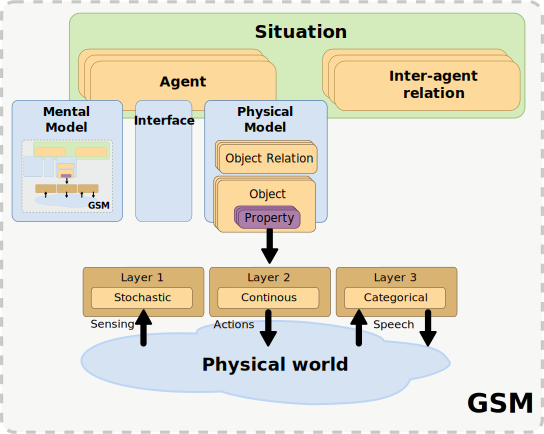
\includegraphics[width=0.65\columnwidth]{stateofart/gsm.pdf}

    \caption{Simplified hierarchical structure of the Grounded Situation Model,
    based on~\cite{Mavridis2006}.}

    \label{fig|gsm}
\end{figure}

Properties are represented in three layers: a stochastic representation, close
to sensory percepts, a \emph{continuous single-valued} encoding of the
stochastic model, and a discrete, categorical model.

One notable feature of GSM is the \emph{bidirectionality} of the grounding
process: not only sensor percepts are abstracted into categories suitable for
human conversation, but human utterance (like ``There is a red ball in the
center of the table'') can also be turned into property descriptions. This
basically enable the knowledge representation system of the robot to
\emph{imagine} entities.

GSM also features several strategies for managing time and events.
\emph{Moments} are created by storing timestamped snap-shots of GSM, and
\emph{event classifiers} allow to define and detect events.

\paragraph{Experiments} GSM has mostly been tested on table-top manipulation
and interaction tasks (a ``conversational helping hand'' as stated by the
authors) implemented on a 7-DOF arm equipped with force feedback, cameras for blob
tracking and speech recognition (Sphinx4). Mavridis and Roy provide in addition
an in-depth analysis of the performance of GSM by the mean of a standard
psycholinguistic test, the \emph{Token test}~\cite{DiSimoni1978}.

\subsection{Ke Jia Project}
\label{sect|kejia}

The Ke Jia project~\cite{Chen2010} integrates on a mobile platform a knowledge
representation language with natural language processing, task planing and
motion planing.

Knowledge representation relies on \emph{Action Language C}, itself based on
\emph{Answer Set Programming} (ASP)~\cite{Gelfond2008}. These languages, that
are syntactically close to Prolog, are based on \emph{stable models} of logic
programs, and support non-monotonic reasoning. Default and non-monotonic
reasoning has been especially researched within the Ke Jia project for symbolic
task planing~\cite{Ji2011} and underspecified natural language processing.

Amongst other features, the natural language processing capabilities of the
system support acquisition of new logical rules at run-time.

\paragraph{Experiments} The Ke Jia robot has been demonstrated in several tasks
involving human-robot interaction with natural language. These tasks include a
task with multiple \emph{pick \& carry} that are globally optimized, naive
physics reasoning via taught rules or more complex scenarii with the robot
delivering drinks, taking into account changing and mutually exclusive
preferences of users.


\subsection{KnowRob}
\label{sect|knowrob}


{\sc KnowRob}~\cite{Tenorth2009a} is an integrated knowledge management system
developed at the Technical University of Munich. It is build as a set of
modules (figure~\ref{fig|knowrob} organized around a core reasoning system
written in Prolog. This core module interfaces through Java/Prolog or
C/Prolog APIs with external modules.

{\sc KnowRob} offers a mechanism called \emph{computables} that allow to
evaluate certain predicates by calling external dedicated functions (for
instance, the valuation of a proposition like \stmt{object1 isOn object2} is
computed when required by calling a specific geometric reasoning module). In
combination with Prolog's lazy evaluation strategy, this supports a good
scalability.

\begin{figure}
    \centering
    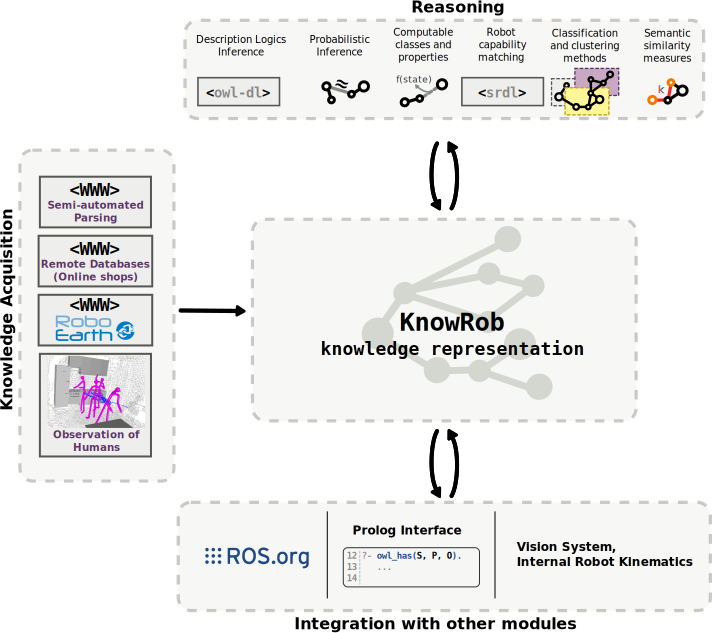
\includegraphics[width=0.7\columnwidth]{stateofart/knowrob.pdf}

    \caption{Overview of the {\sc KnowRob} framework, taken
    from~\cite{Tenorth2011}.}

    \label{fig|knowrob}
\end{figure}

Extension modules can plug into the system to provide specialized reasoning
capabilities or interfaces to external data sources, \eg to read object
detections from the vision system. These modules operate on the level of
instances (ABox).

\paragraph{Knowledge model} {\sc KnowRob} can load OWL ontologies, and the
\emph{KnowRob-Base} ontology is provided as a common-sense ontology, with a
focus on household and kitchen domains. {\sc KnowRob} also store and reason on
introspective knowledge through the \emph{Semantic Robot Description
Language}~\cite{Kunze2011} that allow to represent symbolically the
capabilities of the robot, and is used for planning.


\paragraph{Reasoning Techniques} Amongst the notable {\sc KnowRob} extensions,
{\sc ProbCog}~\cite{Jain2009} is an effort to provide probabilistic reasoning
based on bayesian networks, integration with naive physics reasoning has been
studied~\cite{Kunze2011a}, automatic parsing of Web resources in semi-natural
language has been also experimented with~\cite{Nyga2009}.

\paragraph{Grounding} Anchoring of knowledge in the {\sc KnowRob} framework
relies on...CoP? Semantic Maps~\cite{Blodow2011}.

\fxwarning{to complete}

%\paragraph{Integration with Decisional Layers} CRAM~\cite{Beetz2010}

\paragraph{Notable Experiments} {\sc KnowRob} has been deployed on several
scenarii at the Technical University of Munich, on the PR2 robot and on a 2-arm
custom mobile manipulator in the scope of the ``assistive
kitchen''~\cite{Beetz2008} project. In these experiments, {\sc KnowRob} has
been used as central knowledge hub...
\fxwarning{to complete}

\subsection{NKRL}
\label{sect|nkrl}

\emph{NKRL} stands for \emph{Narrative Knowledge Representation Language}.
While this language is developed since a long time by Zarri~\cite{Zarri1997,
Zarri2008}, recent research direction include application to the robotic
field~\cite{Sabri2011}. NKRL is not {\it per-se} a knowledge representation
system, as it is primarily a language. However, it is used as the
representation and reasoning mechanism for robots by Sabri et al.

\fxwarning{NKRL -> to complete!! (report missing parts to the evaluation table
as well}

\paragraph{Intrinsic language features}
\label{sect|nkrl-intrinsic-features}

Expressiveness...

\paragraph{Integration with physical world and in the robot architecture}
\label{sect|nkrl-integration}

\ldots seem to be mostly WIP\ldots

\subsection{OUR-K and OMRKF}
\label{sect|omrkf}

The Ontology-based Unified Robot Knowledge~\cite{Lim2011} (OUR-K) framework,
successor of the Ontology-based Multi-layered Robot Knowledge
Framework~\cite{Suh2007} (OMRKF), is a knowledge representation system based on
five inter-related \emph{classes} of knowledge (figure~\ref{fig|omrkf}). It
proposes a layered approach to knowledge representation that allows to
integrate the grounding process to the knowledge representation process. OUR-K
knowledge model is implemented with a mix of Description Logics for the concept
hierarchies and Horn clauses.

\begin{figure}
    \centering
    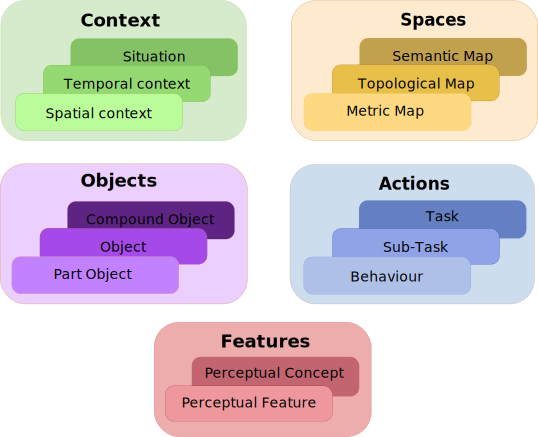
\includegraphics[width=0.5\columnwidth]{stateofart/ourk.pdf}

    \caption{OUR-K organizes knowledge into fives \emph{classes}, each composed
    of \emph{levels}. Figure based on~\cite{Lim2011}.}

    \label{fig|omrkf}
\end{figure}

Each level of knowledge is build as three stages of ontological realization: a
\emph{meta-concept} (the level itself, like ``temporal context'', ``behaviour''
or ``object feature''), a taxonomy of concepts inside this level (for instance
$cup : Object \sqsubseteq tableware : Object$) and an instantiation of the
taxonomy ($cup1 : cup$).

\paragraph{Representation} The environment is represented in OUR-K in the
$spaces : Model$ knowledge level as a classical three layers mapping (metric,
topological and semantic maps). Objects (in $objects : Model$) are localized in
$spaces : Model$ through Voronoi nodes.

The knowledge class $Context$ proposes an explicit statement of spatial context
(mostly geometric relations between objects), temporal context and a more
general \emph{high-level} context, inferred from spatial and temporal contexts.

Finally, the $Activity$ knowledge class store compound actions in a HTN-like
structure, exploited at run-time by a planner.

\fxwarning{re-read the paper to improve the section...}

\paragraph{Experiments} Experiments conducted with OUR-K and OMRKF include
finding kitchen objects and reporting about their state to a human.  This
experiment also shows how OUR-K can deal with objects only partially matched by
their descriptor by introducing a $candidate()$ function.

\subsection{PEIS KR\&R}
\label{sect|peis-ecology}

{\sc PEIS Ecology}~\cite{Saffiotti2005} is a software \emph{ecosystem} that aim
to binds autonomous robotics with ambient intelligence (network of sensors).
\emph{PEIS} stands for \emph{Physically Embedded Intelligent System}: every
robots or intelligent device in the environment is abstracted as a PEIS.

Each PEIS physical component is running a \emph{PEIS Kernel} instance.
Communication between instance relies on a custom P2P communication protocol.

The PEIS architecture allows for adding new abilities through software
components sharing the common \emph{tuple space}.

We consider here the semantic layer~\cite{Daoutis2009}, referred as \emph{PEIS
KR\&R}, that includes symbolic representation and reasoning.

\fxwarning{have a look to latest Daoutis paper!}

% More in details:
% - object identification based on viewpoint independent SIFT features
% - formalized anchoring system that explicitly match percieved attributes to predicates
% - Cyc predicates
% - ground 12 colors, based on a paper on color perception. Could be useful for us.
% - idem, they cite a paper on what spatial relations to compute
% - location of objects based on a previously provided semantic map (but not much on this semantic map)
% - two "memories": the robot memory stores the current list of percieved objects ; the archive memory stores what is not percieved anymore
% - uses directly Cyc (ie, 250 000 common sense concepts\ldots), via CycL language -> 2nd and higher order logics (quantification over predicates, functions, etc)
% Remark: using 2nd order logic (ie meta statements), it would be easy to store the knowledge of each agent
% - disambiguation in concept name by asking human to decide amongst all concepts known by Cyc
% - template based natural language
% - experiment conducted in a "smart" indoor environmement + simple robot

\paragraph{Knowledge model} The PEIS Knowledge representation system relies on
the {\sc ResearchCyc} and {\sc CycL} language to represent knowledge. The {\sc CycL} language
allows to represent first order logic sentences and has extensions for modal logics and higher order logics.

\fxfatal{Is modal logics and higher order logics actually used in PEIS?} 

As a system relying on {\sc CycL}, contexts can be expressed as
\emph{microtheories}: the truth or falsity of a set of statement depends of the
\emph{microtheory} in which these statements are evaluated.

\fxfatal{OWA/CWA?}

\begin{figure}
	\centering
	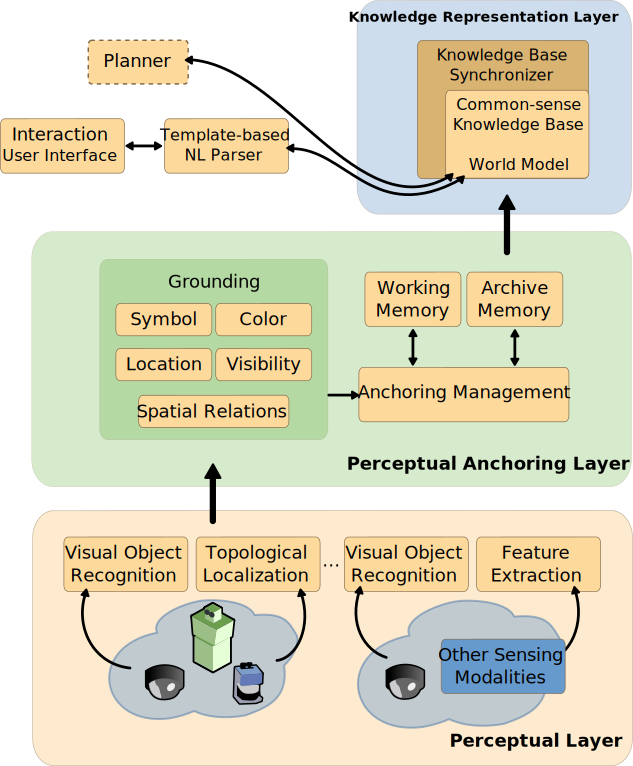
\includegraphics[width=0.5\columnwidth]{stateofart/peis-architecture.pdf}
	\caption{The PEIS knowledge representation system, taken from~\cite{Daoutis2009}}
	\label{fig|peis-archi}
\end{figure}

The PEIS KR\&R system is deeply integrated to the general PEIS Ecology
\emph{smart} environment. Figure~\ref{fig|peis-archi} gives an overview of the
interactions between PEIS knowledge processing layers.

\paragraph{Knowledge Acquisition} The primary source for knowledge acquisition
is perception.  The PEIS ecosystem provides a SIFT-based object recognizer used
in conjunction with ceiling cameras for object localization.  Other perceptual
modalities are available (like human tracking, ambient environment monitoring).

A template-based natural language parsing system may also be used to add new
assertions to the system.

The system can ask the human for help to disambiguate between concept names.

\paragraph{Anchoring} Daoutis et al. formalize the issue of anchoring as
finding a \emph{predicate grounding relation} $g \subseteq \mathcal{P} \times
\Phi \times D(\Phi)$, where $\mathcal{P}$ is a set of predicate symbols, $\Phi$
a set of percept's attributes, and $D(\Phi)$ the domain of these attributes.

In the current implementation, object category (returned by the SIFT
classifier), color, location, spatial relations (both topological -- \emph{at},
\emph{near} -- and relative to the robot -- \emph{left}, \emph{behind}, etc.)
and visibility are the five classes of extracted attributes.

\paragraph{Integration in the robot architecture}
\label{sect|peis-integration}

The PEIS framework offers through the \emph{PEIS middleware} a practical way to
insert a new component into the shared \emph{tuple space}.  Thus, the KR\&R
module can be seamlessly integrated into the PEIS ecosystem.

\paragraph{Experiments}
\label{sect|peis-expe}

\fxwarning{PEIS experiments: TDB}


%%%%%%%%%%%%%%%%%%%%%%%%%%%%%%%%%%%%%%%%%%%%%%%%%%%%%%%%%%%%%%%%%%%%%%%%%%%%%%%

\section{An Interface for Knowledge Manipulation in Robotics}
\label{sect|knowledge-api}

During the preparation of the thesis, discussions with several people involved
in knowledge representation (namely Dominik Jain, Lars Kunze, Michael Beetz)
have led to the draft of a generic API for knowledge access and exchange
between robotics components.

This section presents this effort of standardisation that is (partially)
implemented by the ORO server, presented in the next chapter.

\subsection{Rationale and General Considerations}

The original idea comes from the acknowledgement that more and more software
components for robotics want to store or use symbolic data. Since established
international efforts at defining standard for inter-component communication
like ROS have already proved their usefulness, one single API for different
knowledge representation and management systems could be equally useful.

Two main previous attempts must be mentioned: the \emph{Knowledge Interchange
Format} (KIF) and the DIG interface.

\fxfatal{Complete this part}
The \href{http://dig.sourceforge.net/}{ DIG interface}

The \href{http://logic.stanford.edu/kif/dpans.html}{ Knowledge Interface Format
(KIF)}. In~\cite{Ginsberg1991}, Ginsberg explains why \emph{knowledge
interchange formats} are hardly a good idea.

The API is designed for robotics (even if probably useful in other contexts):
it aims to be simple and practical for clients by focusing on core knowledge
operations (addition of knowledge, retraction, querying) with consistency
constraints; it explicitly supports uncertain knowledge and multiple models
(modality); it makes clear how knowledge is added or retracted with explicit
policies.

We have attempted to design it in a way that do not restrict expressiveness
(any logical sentence that can be expressed in the logic of predicates, with a
probabilistic extension, can be manipulated by the API), and a simple extension
mechanism should permit future evolutions in a backward compatible way.

Besides facilitating exchange of knowledge contents between systems by ensuring
one standard formalism, another outcome of the adoption by several KRS of this
API is that it allows easy switch between semantic engines (and thus
benchmarking and sharing of unit-tests).

This API was developed with Prolog-based knowledge systems, Description
Logics-based knowledge bases and Markov networks in mind, and should cover as
well other systems related to predicate logics (with or without a probabilistic
extension).

Besides standard operations on axioms and taxonomy, the API aims to cover:

\begin{itemize}
    \item  probabilities associated to statements
    \item  management of several models
    \item  explicit policies to add, retract or, more generally, alter 
    knowledge (for instance, to guarantee consistency when adding knowledge)
    \item  specific, implementation-dependent, extensions through the
    \texttt{special} method.
\end{itemize}

Implementations are not always expected to cover to whole API, but must have a
predicable behaviour when a part of the API is not implemented. In particular,
the API makes no assumptions on implementations regarding:

\begin{itemize}
    \item  the actual supported expressiveness (the API allows to express
    general first-order logics statements, but the underlying implementation
    may support only a subset, for instance, Description Logics)
    \item  Closed-world assumption vs Open-world assumption
    \item  Reasoning capabilities
\end{itemize}

\subsection{The Knowledge API}

The API is divided in five parts:
\begin{enumerate}
    \item Methods related to service management,
    \item Methods related to knowledge alteration,
    \item Methods related to knowledge querying,
    \item Methods related to models manipulation and finally
    \item Methods related to taxonomy walking.
\end{enumerate}

Parts 2 and 3 are the two main parts, involved with knowledge manipulation.

\paragraph{Knowledge Alteration} Methods in part 2 are build around the generic
\jmeth{revision} method, that takes as parameter a set of logical propositions
and a policy.

A policy is represented as a set of \texttt{(key, value)} pairs whose possible
values are presented in table~\ref{table|knowledge-policies}.

\begin{table}
\begin{center}

    \begin{tabular}{lp{4cm}p{9cm}}
    \toprule
    Key & Values & Meaning \\
    
    \midrule

    { \tt method} & {\tt add} \emph{(default)} & the statements are added to the
    knowledge base, without ensuring consistency.\\ 
    
    \midrule

    & {\tt safe\_add} & the statements are added only if they (individually) do
    not lead to inconsistencies.\\ 

    \midrule
    
    & {\tt retract} & the statements are removed from the model. Associated
    probabilities are discarded.\\ 
    
    \midrule
    
    &{\tt update} & Updates objects of one or several statements in the
    specified model. If the predicate is not inferred to be \emph{functional}
    (\ie, it accept only one single value), behaves like {\tt add}.\\ 
    
    \midrule
    
    & {\tt revision} or {\tt safe\_update} & Updates objects of one or several
    statements in the specified model if it does not (individually) lead to
    inconsistencies. If the predicate is not inferred to be \emph{functional}
    (\ie, it accepts only one single value), behaves like {\tt safe\_add}.\\ 
    
    \midrule
    
    {\tt model} & {\tt all} \emph{(default)} & all existing \emph{models}
    (section~\ref{sect|kbapi-models}) are impacted by the change.\\

    \midrule
    
    & a valid model id or a set of valid model id & only the specified model(s)
    are impacted\\
    
    \bottomrule
    
    \end{tabular}

\end{center}
\caption{Knowledge revision policies.}
\label{table|knowledge-policies}
\end{table}

\paragraph{Knowledge Querying} The main method that allow for knowledge
retrieval is \jmeth{find}. A \jmeth{find} query is build as a set of partial
statements (\ie, statements with named or anonymous unbound terms) that form a
pattern. It returns statements matching the pattern.

``Shortcut'' methods are offered by the API for common operations
(adding/retracting a statement, checking if a statement exists, etc.). Where
relevant, probabilistic versions of the methods are also defined.

The complete API reference is provided in Appendix~\ref{chapter|kb-api}.


\clearpage

That concludes the chapter on Symbolic Knowledge Representation for robotics.

In that chapter, we have first discussed a definition of \emph{knowledge} in
our context of service robotics and human-robot interaction. We have presented
several references from the literature regarding the identification and
classification of prominent features of knowledge representation systems. 

We have then introduce a comprehensive typology of such features, that
comprises of about fifty concepts sorted into six main categories: features
related to knowledge expressiveness, features related to representation
techniques, features related to reasoning, features related to acquisition and
grounding of knowledge, features related to the integration of a KRS into a
larger robotic architecture, and finally, features that characterize the
represented knowledge itself. Each of the fifty concepts has been briefly
presented with references to the literature.

Finally, we have surveyed nine systems for knowledge representation in service
robots and underlined their main strengths.

The next chapter introduces ORO, a tenth KRS that we have designed and
implemented during the thesis preparation.

